<<<<<<< Updated upstream
% Created by tikzDevice version 0.12.3 on 2021-06-03 00:38:00
=======
% Created by tikzDevice version 0.12.3.1 on 2021-05-07 14:41:55
>>>>>>> Stashed changes
% !TEX encoding = UTF-8 Unicode
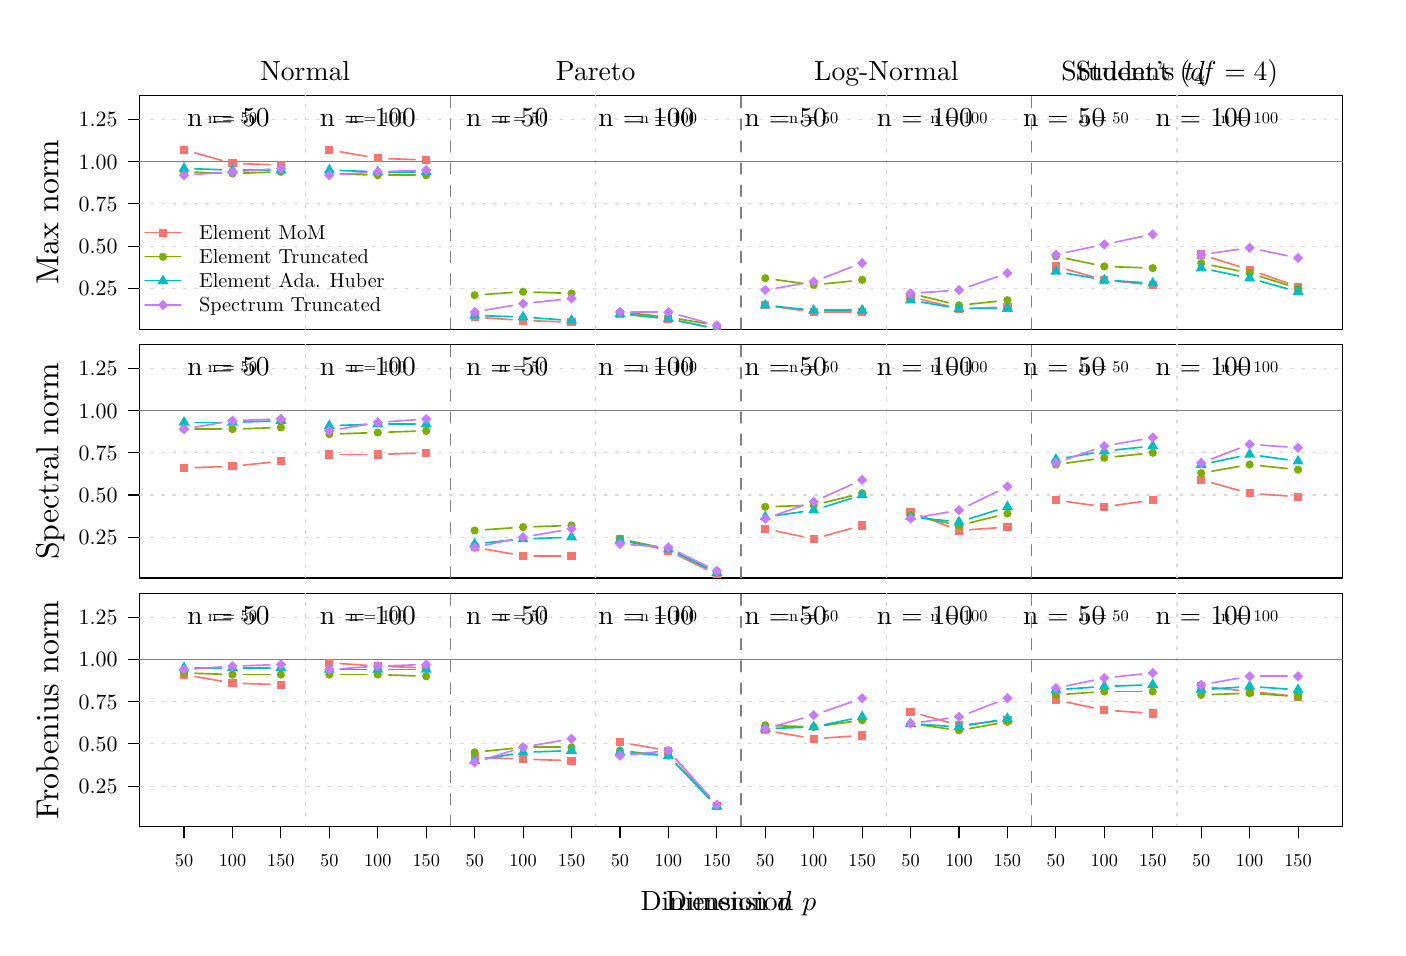
\begin{tikzpicture}[x=1pt,y=1pt]
\definecolor{fillColor}{RGB}{255,255,255}
\path[use as bounding box,fill=fillColor,fill opacity=0.00] (0,0) rectangle (487.82,325.21);
\begin{scope}
\path[clip] (  0.00,  0.00) rectangle (487.82,325.21);
\definecolor{drawColor}{RGB}{0,0,0}

\path[draw=drawColor,line width= 0.4pt,line join=round,line cap=round] ( 40.39,216.28) --
	(475.15,216.28) --
	(475.15,300.66) --
	( 40.39,300.66) --
	( 40.39,216.28);

\path[draw=drawColor,line width= 0.4pt,line join=round,line cap=round] ( 40.39,231.00) -- ( 40.39,292.04);

\path[draw=drawColor,line width= 0.4pt,line join=round,line cap=round] ( 40.39,231.00) -- ( 36.43,231.00);

\path[draw=drawColor,line width= 0.4pt,line join=round,line cap=round] ( 40.39,246.26) -- ( 36.43,246.26);

\path[draw=drawColor,line width= 0.4pt,line join=round,line cap=round] ( 40.39,261.52) -- ( 36.43,261.52);

\path[draw=drawColor,line width= 0.4pt,line join=round,line cap=round] ( 40.39,276.78) -- ( 36.43,276.78);

\path[draw=drawColor,line width= 0.4pt,line join=round,line cap=round] ( 40.39,292.04) -- ( 36.43,292.04);

\node[text=drawColor,anchor=base east,inner sep=0pt, outer sep=0pt, scale=  0.79] at ( 32.47,228.28) {0.25};

\node[text=drawColor,anchor=base east,inner sep=0pt, outer sep=0pt, scale=  0.79] at ( 32.47,243.54) {0.50};

\node[text=drawColor,anchor=base east,inner sep=0pt, outer sep=0pt, scale=  0.79] at ( 32.47,258.80) {0.75};

\node[text=drawColor,anchor=base east,inner sep=0pt, outer sep=0pt, scale=  0.79] at ( 32.47,274.06) {1.00};

\node[text=drawColor,anchor=base east,inner sep=0pt, outer sep=0pt, scale=  0.79] at ( 32.47,289.32) {1.25};
\end{scope}
\begin{scope}
\path[clip] ( 40.39,216.28) rectangle (475.15,300.66);
\definecolor{drawColor}{gray}{0.85}

\path[draw=drawColor,line width= 0.4pt,dash pattern=on 1pt off 3pt ,line join=round,line cap=round] ( 40.39,231.00) -- (475.15,231.00);

\path[draw=drawColor,line width= 0.4pt,dash pattern=on 1pt off 3pt ,line join=round,line cap=round] ( 40.39,246.26) -- (475.15,246.26);

\path[draw=drawColor,line width= 0.4pt,dash pattern=on 1pt off 3pt ,line join=round,line cap=round] ( 40.39,261.52) -- (475.15,261.52);

\path[draw=drawColor,line width= 0.4pt,dash pattern=on 1pt off 3pt ,line join=round,line cap=round] ( 40.39,276.78) -- (475.15,276.78);

\path[draw=drawColor,line width= 0.4pt,dash pattern=on 1pt off 3pt ,line join=round,line cap=round] ( 40.39,292.04) -- (475.15,292.04);

\path[draw=drawColor,line width= 0.4pt,dash pattern=on 1pt off 3pt ,line join=round,line cap=round] (100.25,216.28) -- (100.25,300.66);

\path[draw=drawColor,line width= 0.4pt,dash pattern=on 1pt off 3pt ,line join=round,line cap=round] (205.26,216.28) -- (205.26,300.66);

\path[draw=drawColor,line width= 0.4pt,dash pattern=on 1pt off 3pt ,line join=round,line cap=round] (310.28,216.28) -- (310.28,300.66);

\path[draw=drawColor,line width= 0.4pt,dash pattern=on 1pt off 3pt ,line join=round,line cap=round] (415.29,216.28) -- (415.29,300.66);
\definecolor{drawColor}{gray}{0.50}

\path[draw=drawColor,line width= 0.4pt,dash pattern=on 4pt off 4pt ,line join=round,line cap=round] (152.76,216.28) -- (152.76,300.66);

\path[draw=drawColor,line width= 0.4pt,dash pattern=on 4pt off 4pt ,line join=round,line cap=round] (257.77,216.28) -- (257.77,300.66);

\path[draw=drawColor,line width= 0.4pt,dash pattern=on 4pt off 4pt ,line join=round,line cap=round] (362.79,216.28) -- (362.79,300.66);
\end{scope}
\begin{scope}
\path[clip] (  0.00,  0.00) rectangle (487.82,325.21);
\definecolor{drawColor}{RGB}{0,0,0}

\node[text=drawColor,rotate= 90.00,anchor=base,inner sep=0pt, outer sep=0pt, scale=  1.15] at ( 11.09,258.47) {Max norm};
\end{scope}
\begin{scope}
\path[clip] ( 40.39,216.28) rectangle (475.15,300.66);
\definecolor{drawColor}{gray}{0.50}

\path[draw=drawColor,line width= 0.4pt,line join=round,line cap=round] ( 40.39,276.78) -- (475.15,276.78);
\end{scope}
\begin{scope}
\path[clip] (  0.00,  0.00) rectangle (487.82,325.21);
\definecolor{drawColor}{RGB}{0,0,0}

\node[text=drawColor,anchor=base,inner sep=0pt, outer sep=0pt, scale=  1.00] at (100.25,306.21) {Normal};

\node[text=drawColor,anchor=base,inner sep=0pt, outer sep=0pt, scale=  1.00] at (205.26,306.21) {Pareto};

\node[text=drawColor,anchor=base,inner sep=0pt, outer sep=0pt, scale=  1.00] at (310.28,306.21) {Log-Normal};

<<<<<<< Updated upstream
\node[text=drawColor,anchor=base,inner sep=0pt, outer sep=0pt, scale=  1.00] at (415.29,306.21) {Student ($df = 4$)};
=======
\node[text=drawColor,anchor=base,inner sep=0pt, outer sep=0pt, scale=  1.00] at (399.71,306.21) {Student's $t_4$};
>>>>>>> Stashed changes
\end{scope}
\begin{scope}
\path[clip] ( 40.39,216.28) rectangle (475.15,300.66);
\definecolor{drawColor}{RGB}{0,0,0}

<<<<<<< Updated upstream
\node[text=drawColor,anchor=base,inner sep=0pt, outer sep=0pt, scale=  0.59] at ( 74.00,290.43) {n = 50};

\node[text=drawColor,anchor=base,inner sep=0pt, outer sep=0pt, scale=  0.59] at (126.50,290.43) {n = 100};

\node[text=drawColor,anchor=base,inner sep=0pt, outer sep=0pt, scale=  0.59] at (179.01,290.43) {n = 50};

\node[text=drawColor,anchor=base,inner sep=0pt, outer sep=0pt, scale=  0.59] at (231.52,290.43) {n = 100};

\node[text=drawColor,anchor=base,inner sep=0pt, outer sep=0pt, scale=  0.59] at (284.02,290.43) {n = 50};

\node[text=drawColor,anchor=base,inner sep=0pt, outer sep=0pt, scale=  0.59] at (336.53,290.43) {n = 100};

\node[text=drawColor,anchor=base,inner sep=0pt, outer sep=0pt, scale=  0.59] at (389.04,290.43) {n = 50};

\node[text=drawColor,anchor=base,inner sep=0pt, outer sep=0pt, scale=  0.59] at (441.55,290.43) {n = 100};
=======
\node[text=drawColor,anchor=base,inner sep=0pt, outer sep=0pt, scale=  0.99] at ( 72.60,289.35) {n = 50};

\node[text=drawColor,anchor=base,inner sep=0pt, outer sep=0pt, scale=  0.99] at (122.92,289.35) {n = 100};

\node[text=drawColor,anchor=base,inner sep=0pt, outer sep=0pt, scale=  0.99] at (173.25,289.35) {n = 50};

\node[text=drawColor,anchor=base,inner sep=0pt, outer sep=0pt, scale=  0.99] at (223.57,289.35) {n = 100};

\node[text=drawColor,anchor=base,inner sep=0pt, outer sep=0pt, scale=  0.99] at (273.90,289.35) {n = 50};

\node[text=drawColor,anchor=base,inner sep=0pt, outer sep=0pt, scale=  0.99] at (324.22,289.35) {n = 100};

\node[text=drawColor,anchor=base,inner sep=0pt, outer sep=0pt, scale=  0.99] at (374.55,289.35) {n = 50};

\node[text=drawColor,anchor=base,inner sep=0pt, outer sep=0pt, scale=  0.99] at (424.87,289.35) {n = 100};
>>>>>>> Stashed changes
\definecolor{drawColor}{RGB}{248,118,109}

\path[draw=drawColor,line width= 0.4pt,line join=round,line cap=round] ( 42.35,251.13) -- ( 55.42,251.13);
\definecolor{drawColor}{RGB}{124,174,0}

\path[draw=drawColor,line width= 0.4pt,line join=round,line cap=round] ( 42.35,242.42) -- ( 55.42,242.42);
\definecolor{drawColor}{RGB}{0,191,196}

\path[draw=drawColor,line width= 0.4pt,line join=round,line cap=round] ( 42.35,233.71) -- ( 55.42,233.71);
\definecolor{drawColor}{RGB}{199,124,255}

\path[draw=drawColor,line width= 0.4pt,line join=round,line cap=round] ( 42.35,224.99) -- ( 55.42,224.99);
\definecolor{fillColor}{RGB}{248,118,109}

\path[fill=fillColor] ( 47.40,249.64) --
	( 50.37,249.64) --
	( 50.37,252.61) --
	( 47.40,252.61) --
	cycle;
\definecolor{fillColor}{RGB}{124,174,0}

\path[fill=fillColor] ( 48.89,242.42) circle (  1.48);
\definecolor{fillColor}{RGB}{0,191,196}

\path[fill=fillColor] ( 48.89,236.02) --
	( 50.89,232.55) --
	( 46.89,232.55) --
	cycle;
\definecolor{fillColor}{RGB}{199,124,255}

\path[fill=fillColor] ( 47.03,224.99) --
	( 48.89,226.85) --
	( 50.74,224.99) --
	( 48.89,223.14) --
	cycle;
\definecolor{drawColor}{RGB}{0,0,0}

\node[text=drawColor,anchor=base west,inner sep=0pt, outer sep=0pt, scale=  0.73] at ( 61.95,248.63) {Element MoM};

\node[text=drawColor,anchor=base west,inner sep=0pt, outer sep=0pt, scale=  0.73] at ( 61.95,239.92) {Element Truncated};

\node[text=drawColor,anchor=base west,inner sep=0pt, outer sep=0pt, scale=  0.73] at ( 61.95,231.21) {Element Ada. Huber};

\node[text=drawColor,anchor=base west,inner sep=0pt, outer sep=0pt, scale=  0.73] at ( 61.95,222.49) {Spectrum Truncated};
\definecolor{drawColor}{RGB}{248,118,109}

\path[draw=drawColor,line width= 0.6pt,line join=round,line cap=round] ( 60.31,279.99) -- ( 70.18,277.24);

\path[draw=drawColor,line width= 0.6pt,line join=round,line cap=round] ( 77.95,276.04) -- ( 87.54,275.70);
\definecolor{fillColor}{RGB}{248,118,109}

\path[fill=fillColor] ( 55.01,279.57) --
	( 57.98,279.57) --
	( 57.98,282.54) --
	( 55.01,282.54) --
	cycle;

\path[fill=fillColor] ( 72.51,274.69) --
	( 75.48,274.69) --
	( 75.48,277.66) --
	( 72.51,277.66) --
	cycle;

\path[fill=fillColor] ( 90.01,274.08) --
	( 92.98,274.08) --
	( 92.98,277.05) --
	( 90.01,277.05) --
	cycle;
\definecolor{drawColor}{RGB}{124,174,0}

\path[draw=drawColor,line width= 0.6pt,line join=round,line cap=round] ( 60.45,272.98) -- ( 70.04,272.65);

\path[draw=drawColor,line width= 0.6pt,line join=round,line cap=round] ( 77.95,272.65) -- ( 87.54,272.98);
\definecolor{fillColor}{RGB}{124,174,0}

\path[fill=fillColor] ( 56.49,273.12) circle (  1.48);

\path[fill=fillColor] ( 74.00,272.51) circle (  1.48);

\path[fill=fillColor] ( 91.50,273.12) circle (  1.48);
\definecolor{drawColor}{RGB}{0,191,196}

\path[draw=drawColor,line width= 0.6pt,line join=round,line cap=round] ( 60.45,274.20) -- ( 70.04,273.87);

\path[draw=drawColor,line width= 0.6pt,line join=round,line cap=round] ( 77.96,273.73) -- ( 87.54,273.73);
\definecolor{fillColor}{RGB}{0,191,196}

\path[fill=fillColor] ( 56.49,276.65) --
	( 58.49,273.19) --
	( 54.49,273.19) --
	cycle;

\path[fill=fillColor] ( 74.00,276.04) --
	( 76.00,272.58) --
	( 72.00,272.58) --
	cycle;

\path[fill=fillColor] ( 91.50,276.04) --
	( 93.50,272.58) --
	( 89.50,272.58) --
	cycle;
\definecolor{drawColor}{RGB}{199,124,255}

\path[draw=drawColor,line width= 0.6pt,line join=round,line cap=round] ( 60.44,272.18) -- ( 70.05,272.85);

\path[draw=drawColor,line width= 0.6pt,line join=round,line cap=round] ( 77.95,273.40) -- ( 87.55,274.07);
\definecolor{fillColor}{RGB}{199,124,255}

\path[fill=fillColor] ( 54.64,271.90) --
	( 56.49,273.76) --
	( 58.35,271.90) --
	( 56.49,270.04) --
	cycle;

\path[fill=fillColor] ( 72.14,273.12) --
	( 74.00,274.98) --
	( 75.85,273.12) --
	( 74.00,271.27) --
	cycle;

\path[fill=fillColor] ( 89.64,274.34) --
	( 91.50,276.20) --
	( 93.36,274.34) --
	( 91.50,272.49) --
	cycle;
\definecolor{drawColor}{RGB}{248,118,109}

\path[draw=drawColor,line width= 0.6pt,line join=round,line cap=round] (112.90,280.38) -- (122.60,278.69);

\path[draw=drawColor,line width= 0.6pt,line join=round,line cap=round] (130.46,277.87) -- (140.05,277.53);
\definecolor{fillColor}{RGB}{248,118,109}

\path[fill=fillColor] (107.52,279.57) --
	(110.49,279.57) --
	(110.49,282.54) --
	(107.52,282.54) --
	cycle;

\path[fill=fillColor] (125.02,276.52) --
	(127.99,276.52) --
	(127.99,279.49) --
	(125.02,279.49) --
	cycle;

\path[fill=fillColor] (142.52,275.91) --
	(145.49,275.91) --
	(145.49,278.88) --
	(142.52,278.88) --
	cycle;
\definecolor{drawColor}{RGB}{124,174,0}

\path[draw=drawColor,line width= 0.6pt,line join=round,line cap=round] (112.96,272.37) -- (122.55,272.04);

\path[draw=drawColor,line width= 0.6pt,line join=round,line cap=round] (130.46,271.90) -- (140.05,271.90);
\definecolor{fillColor}{RGB}{124,174,0}

\path[fill=fillColor] (109.00,272.51) circle (  1.48);

\path[fill=fillColor] (126.50,271.90) circle (  1.48);

\path[fill=fillColor] (144.01,271.90) circle (  1.48);
\definecolor{drawColor}{RGB}{0,191,196}

\path[draw=drawColor,line width= 0.6pt,line join=round,line cap=round] (112.96,273.59) -- (122.55,273.26);

\path[draw=drawColor,line width= 0.6pt,line join=round,line cap=round] (130.46,273.12) -- (140.05,273.12);
\definecolor{fillColor}{RGB}{0,191,196}

\path[fill=fillColor] (109.00,276.04) --
	(111.00,272.58) --
	(107.00,272.58) --
	cycle;

\path[fill=fillColor] (126.50,275.43) --
	(128.50,271.97) --
	(124.50,271.97) --
	cycle;

\path[fill=fillColor] (144.01,275.43) --
	(146.01,271.97) --
	(142.01,271.97) --
	cycle;
\definecolor{drawColor}{RGB}{199,124,255}

\path[draw=drawColor,line width= 0.6pt,line join=round,line cap=round] (112.95,272.18) -- (122.55,272.85);

\path[draw=drawColor,line width= 0.6pt,line join=round,line cap=round] (130.46,273.26) -- (140.05,273.59);
\definecolor{fillColor}{RGB}{199,124,255}

\path[fill=fillColor] (107.14,271.90) --
	(109.00,273.76) --
	(110.86,271.90) --
	(109.00,270.04) --
	cycle;

\path[fill=fillColor] (124.65,273.12) --
	(126.50,274.98) --
	(128.36,273.12) --
	(126.50,271.27) --
	cycle;

\path[fill=fillColor] (142.15,273.73) --
	(144.01,275.59) --
	(145.86,273.73) --
	(144.01,271.88) --
	cycle;
\definecolor{drawColor}{RGB}{248,118,109}

\path[draw=drawColor,line width= 0.6pt,line join=round,line cap=round] (165.46,220.35) -- (175.06,219.68);

\path[draw=drawColor,line width= 0.6pt,line join=round,line cap=round] (182.97,219.27) -- (192.56,218.93);
\definecolor{fillColor}{RGB}{248,118,109}

\path[fill=fillColor] (160.02,219.14) --
	(162.99,219.14) --
	(162.99,222.11) --
	(160.02,222.11) --
	cycle;

\path[fill=fillColor] (177.53,217.92) --
	(180.50,217.92) --
	(180.50,220.89) --
	(177.53,220.89) --
	cycle;

\path[fill=fillColor] (195.03,217.31) --
	(198.00,217.31) --
	(198.00,220.28) --
	(195.03,220.28) --
	cycle;
\definecolor{drawColor}{RGB}{124,174,0}

\path[draw=drawColor,line width= 0.6pt,line join=round,line cap=round] (165.46,228.84) -- (175.06,229.51);

\path[draw=drawColor,line width= 0.6pt,line join=round,line cap=round] (182.97,229.65) -- (192.56,229.31);
\definecolor{fillColor}{RGB}{124,174,0}

\path[fill=fillColor] (161.51,228.56) circle (  1.48);

\path[fill=fillColor] (179.01,229.78) circle (  1.48);

\path[fill=fillColor] (196.51,229.17) circle (  1.48);
\definecolor{drawColor}{RGB}{0,191,196}

\path[draw=drawColor,line width= 0.6pt,line join=round,line cap=round] (165.47,221.10) -- (175.05,220.77);

\path[draw=drawColor,line width= 0.6pt,line join=round,line cap=round] (182.96,220.35) -- (192.56,219.68);
\definecolor{fillColor}{RGB}{0,191,196}

\path[fill=fillColor] (161.51,223.55) --
	(163.51,220.08) --
	(159.51,220.08) --
	cycle;

\path[fill=fillColor] (179.01,222.94) --
	(181.01,219.47) --
	(177.01,219.47) --
	cycle;

\path[fill=fillColor] (196.51,221.72) --
	(198.51,218.25) --
	(194.51,218.25) --
	cycle;
\definecolor{drawColor}{RGB}{199,124,255}

\path[draw=drawColor,line width= 0.6pt,line join=round,line cap=round] (165.41,223.14) -- (175.11,224.83);

\path[draw=drawColor,line width= 0.6pt,line join=round,line cap=round] (182.95,225.92) -- (192.57,226.93);
\definecolor{fillColor}{RGB}{199,124,255}

\path[fill=fillColor] (159.65,222.46) --
	(161.51,224.32) --
	(163.36,222.46) --
	(161.51,220.60) --
	cycle;

\path[fill=fillColor] (177.15,225.51) --
	(179.01,227.37) --
	(180.87,225.51) --
	(179.01,223.65) --
	cycle;

\path[fill=fillColor] (194.66,227.34) --
	(196.51,229.20) --
	(198.37,227.34) --
	(196.51,225.49) --
	cycle;
\definecolor{drawColor}{RGB}{248,118,109}

\path[draw=drawColor,line width= 0.6pt,line join=round,line cap=round] (217.95,221.44) -- (227.58,220.43);

\path[draw=drawColor,line width= 0.6pt,line join=round,line cap=round] (235.39,219.21) -- (245.14,217.17);
\definecolor{fillColor}{RGB}{248,118,109}

\path[fill=fillColor] (212.53,220.36) --
	(215.50,220.36) --
	(215.50,223.33) --
	(212.53,223.33) --
	cycle;

\path[fill=fillColor] (230.03,218.53) --
	(233.00,218.53) --
	(233.00,221.50) --
	(230.03,221.50) --
	cycle;

\path[fill=fillColor] (247.54,214.87) --
	(250.51,214.87) --
	(250.51,217.84) --
	(247.54,217.84) --
	cycle;
\definecolor{drawColor}{RGB}{124,174,0}

\path[draw=drawColor,line width= 0.6pt,line join=round,line cap=round] (217.95,222.05) -- (227.58,221.04);

\path[draw=drawColor,line width= 0.6pt,line join=round,line cap=round] (235.42,219.95) -- (245.12,218.26);
\definecolor{fillColor}{RGB}{124,174,0}

\path[fill=fillColor] (214.02,222.46) circle (  1.48);

\path[fill=fillColor] (231.52,220.63) circle (  1.48);

\path[fill=fillColor] (249.02,217.58) circle (  1.48);
\definecolor{drawColor}{RGB}{0,191,196}

\path[draw=drawColor,line width= 0.6pt,line join=round,line cap=round] (217.95,221.44) -- (227.58,220.43);

\path[draw=drawColor,line width= 0.6pt,line join=round,line cap=round] (235.39,219.21) -- (245.14,217.17);
\definecolor{fillColor}{RGB}{0,191,196}

\path[fill=fillColor] (214.02,224.16) --
	(216.02,220.69) --
	(212.02,220.69) --
	cycle;

\path[fill=fillColor] (231.52,222.33) --
	(233.52,218.86) --
	(229.52,218.86) --
	cycle;

\path[fill=fillColor] (249.02,218.66) --
	(251.02,215.20) --
	(247.02,215.20) --
	cycle;
\definecolor{drawColor}{RGB}{199,124,255}

\path[draw=drawColor,line width= 0.6pt,line join=round,line cap=round] (217.98,222.46) -- (227.56,222.46);

\path[draw=drawColor,line width= 0.6pt,line join=round,line cap=round] (235.33,221.39) -- (245.21,218.64);
\definecolor{fillColor}{RGB}{199,124,255}

\path[fill=fillColor] (212.16,222.46) --
	(214.02,224.32) --
	(215.87,222.46) --
	(214.02,220.60) --
	cycle;

\path[fill=fillColor] (229.66,222.46) --
	(231.52,224.32) --
	(233.37,222.46) --
	(231.52,220.60) --
	cycle;

\path[fill=fillColor] (247.16,217.58) --
	(249.02,219.43) --
	(250.88,217.58) --
	(249.02,215.72) --
	cycle;
\definecolor{drawColor}{RGB}{248,118,109}

\path[draw=drawColor,line width= 0.6pt,line join=round,line cap=round] (270.44,224.35) -- (280.10,223.01);

\path[draw=drawColor,line width= 0.6pt,line join=round,line cap=round] (287.98,222.46) -- (297.57,222.46);
\definecolor{fillColor}{RGB}{248,118,109}

\path[fill=fillColor] (265.04,223.42) --
	(268.01,223.42) --
	(268.01,226.39) --
	(265.04,226.39) --
	cycle;

\path[fill=fillColor] (282.54,220.97) --
	(285.51,220.97) --
	(285.51,223.94) --
	(282.54,223.94) --
	cycle;

\path[fill=fillColor] (300.04,220.97) --
	(303.01,220.97) --
	(303.01,223.94) --
	(300.04,223.94) --
	cycle;
\definecolor{drawColor}{RGB}{124,174,0}

\path[draw=drawColor,line width= 0.6pt,line join=round,line cap=round] (270.44,234.12) -- (280.10,232.77);

\path[draw=drawColor,line width= 0.6pt,line join=round,line cap=round] (287.96,232.64) -- (297.59,233.64);
\definecolor{fillColor}{RGB}{124,174,0}

\path[fill=fillColor] (266.52,234.67) circle (  1.48);

\path[fill=fillColor] (284.02,232.23) circle (  1.48);

\path[fill=fillColor] (301.53,234.06) circle (  1.48);
\definecolor{drawColor}{RGB}{0,191,196}

\path[draw=drawColor,line width= 0.6pt,line join=round,line cap=round] (270.46,224.49) -- (280.09,223.48);

\path[draw=drawColor,line width= 0.6pt,line join=round,line cap=round] (287.98,223.07) -- (297.57,223.07);
\definecolor{fillColor}{RGB}{0,191,196}

\path[fill=fillColor] (266.52,227.21) --
	(268.52,223.75) --
	(264.52,223.75) --
	cycle;

\path[fill=fillColor] (284.02,225.38) --
	(286.02,221.91) --
	(282.02,221.91) --
	cycle;

\path[fill=fillColor] (301.53,225.38) --
	(303.53,221.91) --
	(299.53,221.91) --
	cycle;
\definecolor{drawColor}{RGB}{199,124,255}

\path[draw=drawColor,line width= 0.6pt,line join=round,line cap=round] (270.42,231.07) -- (280.12,232.77);

\path[draw=drawColor,line width= 0.6pt,line join=round,line cap=round] (287.72,234.86) -- (297.83,238.74);
\definecolor{fillColor}{RGB}{199,124,255}

\path[fill=fillColor] (264.67,230.39) --
	(266.52,232.25) --
	(268.38,230.39) --
	(266.52,228.54) --
	cycle;

\path[fill=fillColor] (282.17,233.45) --
	(284.02,235.30) --
	(285.88,233.45) --
	(284.02,231.59) --
	cycle;

\path[fill=fillColor] (299.67,240.16) --
	(301.53,242.02) --
	(303.38,240.16) --
	(301.53,238.30) --
	cycle;
\definecolor{drawColor}{RGB}{248,118,109}

\path[draw=drawColor,line width= 0.6pt,line join=round,line cap=round] (322.88,227.01) -- (332.68,224.62);

\path[draw=drawColor,line width= 0.6pt,line join=round,line cap=round] (340.49,223.82) -- (350.08,224.15);
\definecolor{fillColor}{RGB}{248,118,109}

\path[fill=fillColor] (317.54,226.47) --
	(320.51,226.47) --
	(320.51,229.44) --
	(317.54,229.44) --
	cycle;

\path[fill=fillColor] (335.05,222.19) --
	(338.02,222.19) --
	(338.02,225.16) --
	(335.05,225.16) --
	cycle;

\path[fill=fillColor] (352.55,222.81) --
	(355.52,222.81) --
	(355.52,225.78) --
	(352.55,225.78) --
	cycle;
\definecolor{drawColor}{RGB}{124,174,0}

\path[draw=drawColor,line width= 0.6pt,line join=round,line cap=round] (322.88,228.23) -- (332.68,225.84);

\path[draw=drawColor,line width= 0.6pt,line join=round,line cap=round] (340.47,225.31) -- (350.10,226.32);
\definecolor{fillColor}{RGB}{124,174,0}

\path[fill=fillColor] (319.03,229.17) circle (  1.48);

\path[fill=fillColor] (336.53,224.90) circle (  1.48);

\path[fill=fillColor] (354.03,226.73) circle (  1.48);
\definecolor{drawColor}{RGB}{0,191,196}

\path[draw=drawColor,line width= 0.6pt,line join=round,line cap=round] (322.93,226.05) -- (332.63,224.36);

\path[draw=drawColor,line width= 0.6pt,line join=round,line cap=round] (340.49,223.68) -- (350.07,223.68);
\definecolor{fillColor}{RGB}{0,191,196}

\path[fill=fillColor] (319.03,229.04) --
	(321.03,225.58) --
	(317.03,225.58) --
	cycle;

\path[fill=fillColor] (336.53,225.99) --
	(338.53,222.53) --
	(334.53,222.53) --
	cycle;

\path[fill=fillColor] (354.03,225.99) --
	(356.03,222.53) --
	(352.03,222.53) --
	cycle;
\definecolor{drawColor}{RGB}{199,124,255}

\path[draw=drawColor,line width= 0.6pt,line join=round,line cap=round] (322.98,229.45) -- (332.58,230.12);

\path[draw=drawColor,line width= 0.6pt,line join=round,line cap=round] (340.27,231.70) -- (350.30,235.19);
\definecolor{fillColor}{RGB}{199,124,255}

\path[fill=fillColor] (317.17,229.17) --
	(319.03,231.03) --
	(320.89,229.17) --
	(319.03,227.32) --
	cycle;

\path[fill=fillColor] (334.68,230.39) --
	(336.53,232.25) --
	(338.39,230.39) --
	(336.53,228.54) --
	cycle;

\path[fill=fillColor] (352.18,236.50) --
	(354.03,238.35) --
	(355.89,236.50) --
	(354.03,234.64) --
	cycle;
\definecolor{drawColor}{RGB}{248,118,109}

\path[draw=drawColor,line width= 0.6pt,line join=round,line cap=round] (375.35,237.88) -- (385.22,235.12);

\path[draw=drawColor,line width= 0.6pt,line join=round,line cap=round] (392.98,233.64) -- (402.60,232.64);
\definecolor{fillColor}{RGB}{248,118,109}

\path[fill=fillColor] (370.05,237.45) --
	(373.02,237.45) --
	(373.02,240.42) --
	(370.05,240.42) --
	cycle;

\path[fill=fillColor] (387.55,232.57) --
	(390.52,232.57) --
	(390.52,235.54) --
	(387.55,235.54) --
	cycle;

\path[fill=fillColor] (405.06,230.74) --
	(408.03,230.74) --
	(408.03,233.71) --
	(405.06,233.71) --
	cycle;
\definecolor{drawColor}{RGB}{124,174,0}

\path[draw=drawColor,line width= 0.6pt,line join=round,line cap=round] (375.41,241.79) -- (385.16,239.75);

\path[draw=drawColor,line width= 0.6pt,line join=round,line cap=round] (393.00,238.80) -- (402.58,238.47);
\definecolor{fillColor}{RGB}{124,174,0}

\path[fill=fillColor] (371.54,242.60) circle (  1.48);

\path[fill=fillColor] (389.04,238.94) circle (  1.48);

\path[fill=fillColor] (406.54,238.33) circle (  1.48);
\definecolor{drawColor}{RGB}{0,191,196}

\path[draw=drawColor,line width= 0.6pt,line join=round,line cap=round] (375.44,236.43) -- (385.14,234.74);

\path[draw=drawColor,line width= 0.6pt,line join=round,line cap=round] (392.99,233.78) -- (402.59,233.11);
\definecolor{fillColor}{RGB}{0,191,196}

\path[fill=fillColor] (371.54,239.42) --
	(373.54,235.95) --
	(369.54,235.95) --
	cycle;

\path[fill=fillColor] (389.04,236.37) --
	(391.04,232.90) --
	(387.04,232.90) --
	cycle;

\path[fill=fillColor] (406.54,235.15) --
	(408.54,231.68) --
	(404.54,231.68) --
	cycle;
\definecolor{drawColor}{RGB}{199,124,255}

\path[draw=drawColor,line width= 0.6pt,line join=round,line cap=round] (375.41,244.02) -- (385.16,246.06);

\path[draw=drawColor,line width= 0.6pt,line join=round,line cap=round] (392.91,247.69) -- (402.67,249.73);
\definecolor{fillColor}{RGB}{199,124,255}

\path[fill=fillColor] (369.68,243.21) --
	(371.54,245.07) --
	(373.39,243.21) --
	(371.54,241.36) --
	cycle;

\path[fill=fillColor] (387.18,246.87) --
	(389.04,248.73) --
	(390.90,246.87) --
	(389.04,245.02) --
	cycle;

\path[fill=fillColor] (404.69,250.54) --
	(406.54,252.39) --
	(408.40,250.54) --
	(406.54,248.68) --
	cycle;
\definecolor{drawColor}{RGB}{248,118,109}

\path[draw=drawColor,line width= 0.6pt,line join=round,line cap=round] (427.82,242.03) -- (437.77,238.90);

\path[draw=drawColor,line width= 0.6pt,line join=round,line cap=round] (445.29,236.42) -- (455.31,232.92);
\definecolor{fillColor}{RGB}{248,118,109}

\path[fill=fillColor] (422.56,241.73) --
	(425.53,241.73) --
	(425.53,244.70) --
	(422.56,244.70) --
	cycle;

\path[fill=fillColor] (440.06,236.23) --
	(443.03,236.23) --
	(443.03,239.20) --
	(440.06,239.20) --
	cycle;

\path[fill=fillColor] (457.56,230.13) --
	(460.53,230.13) --
	(460.53,233.10) --
	(457.56,233.10) --
	cycle;
\definecolor{drawColor}{RGB}{124,174,0}

\path[draw=drawColor,line width= 0.6pt,line join=round,line cap=round] (427.92,239.35) -- (437.67,237.31);

\path[draw=drawColor,line width= 0.6pt,line join=round,line cap=round] (445.32,235.31) -- (455.27,232.19);
\definecolor{fillColor}{RGB}{124,174,0}

\path[fill=fillColor] (424.04,240.16) circle (  1.48);

\path[fill=fillColor] (441.55,236.50) circle (  1.48);

\path[fill=fillColor] (459.05,231.00) circle (  1.48);
\definecolor{drawColor}{RGB}{0,191,196}

\path[draw=drawColor,line width= 0.6pt,line join=round,line cap=round] (427.92,237.52) -- (437.67,235.48);

\path[draw=drawColor,line width= 0.6pt,line join=round,line cap=round] (445.36,233.60) -- (455.23,230.85);
\definecolor{fillColor}{RGB}{0,191,196}

\path[fill=fillColor] (424.04,240.64) --
	(426.04,237.17) --
	(422.04,237.17) --
	cycle;

\path[fill=fillColor] (441.55,236.98) --
	(443.55,233.51) --
	(439.55,233.51) --
	cycle;

\path[fill=fillColor] (459.05,232.09) --
	(461.05,228.63) --
	(457.05,228.63) --
	cycle;
\definecolor{drawColor}{RGB}{199,124,255}

\path[draw=drawColor,line width= 0.6pt,line join=round,line cap=round] (427.97,243.76) -- (437.62,245.11);

\path[draw=drawColor,line width= 0.6pt,line join=round,line cap=round] (445.42,244.84) -- (455.17,242.80);
\definecolor{fillColor}{RGB}{199,124,255}

\path[fill=fillColor] (422.19,243.21) --
	(424.04,245.07) --
	(425.90,243.21) --
	(424.04,241.36) --
	cycle;

\path[fill=fillColor] (439.69,245.65) --
	(441.55,247.51) --
	(443.40,245.65) --
	(441.55,243.80) --
	cycle;

\path[fill=fillColor] (457.19,241.99) --
	(459.05,243.85) --
	(460.90,241.99) --
	(459.05,240.14) --
	cycle;
\end{scope}
\begin{scope}
\path[clip] (  0.00,  0.00) rectangle (487.82,325.21);
\definecolor{drawColor}{RGB}{0,0,0}

\path[draw=drawColor,line width= 0.4pt,line join=round,line cap=round] ( 40.39,126.36) --
	(475.15,126.36) --
	(475.15,210.74) --
	( 40.39,210.74) --
	( 40.39,126.36);

\path[draw=drawColor,line width= 0.4pt,line join=round,line cap=round] ( 40.39,141.08) -- ( 40.39,202.12);

\path[draw=drawColor,line width= 0.4pt,line join=round,line cap=round] ( 40.39,141.08) -- ( 36.43,141.08);

\path[draw=drawColor,line width= 0.4pt,line join=round,line cap=round] ( 40.39,156.34) -- ( 36.43,156.34);

\path[draw=drawColor,line width= 0.4pt,line join=round,line cap=round] ( 40.39,171.60) -- ( 36.43,171.60);

\path[draw=drawColor,line width= 0.4pt,line join=round,line cap=round] ( 40.39,186.86) -- ( 36.43,186.86);

\path[draw=drawColor,line width= 0.4pt,line join=round,line cap=round] ( 40.39,202.12) -- ( 36.43,202.12);

\node[text=drawColor,anchor=base east,inner sep=0pt, outer sep=0pt, scale=  0.79] at ( 32.47,138.35) {0.25};

\node[text=drawColor,anchor=base east,inner sep=0pt, outer sep=0pt, scale=  0.79] at ( 32.47,153.61) {0.50};

\node[text=drawColor,anchor=base east,inner sep=0pt, outer sep=0pt, scale=  0.79] at ( 32.47,168.87) {0.75};

\node[text=drawColor,anchor=base east,inner sep=0pt, outer sep=0pt, scale=  0.79] at ( 32.47,184.13) {1.00};

\node[text=drawColor,anchor=base east,inner sep=0pt, outer sep=0pt, scale=  0.79] at ( 32.47,199.39) {1.25};
\end{scope}
\begin{scope}
\path[clip] ( 40.39,126.36) rectangle (475.15,210.74);
\definecolor{drawColor}{gray}{0.85}

\path[draw=drawColor,line width= 0.4pt,dash pattern=on 1pt off 3pt ,line join=round,line cap=round] ( 40.39,141.08) -- (475.15,141.08);

\path[draw=drawColor,line width= 0.4pt,dash pattern=on 1pt off 3pt ,line join=round,line cap=round] ( 40.39,156.34) -- (475.15,156.34);

\path[draw=drawColor,line width= 0.4pt,dash pattern=on 1pt off 3pt ,line join=round,line cap=round] ( 40.39,171.60) -- (475.15,171.60);

\path[draw=drawColor,line width= 0.4pt,dash pattern=on 1pt off 3pt ,line join=round,line cap=round] ( 40.39,186.86) -- (475.15,186.86);

\path[draw=drawColor,line width= 0.4pt,dash pattern=on 1pt off 3pt ,line join=round,line cap=round] ( 40.39,202.12) -- (475.15,202.12);

\path[draw=drawColor,line width= 0.4pt,dash pattern=on 1pt off 3pt ,line join=round,line cap=round] (100.25,126.36) -- (100.25,210.74);

\path[draw=drawColor,line width= 0.4pt,dash pattern=on 1pt off 3pt ,line join=round,line cap=round] (205.26,126.36) -- (205.26,210.74);

\path[draw=drawColor,line width= 0.4pt,dash pattern=on 1pt off 3pt ,line join=round,line cap=round] (310.28,126.36) -- (310.28,210.74);

\path[draw=drawColor,line width= 0.4pt,dash pattern=on 1pt off 3pt ,line join=round,line cap=round] (415.29,126.36) -- (415.29,210.74);
\definecolor{drawColor}{gray}{0.50}

\path[draw=drawColor,line width= 0.4pt,dash pattern=on 4pt off 4pt ,line join=round,line cap=round] (152.76,126.36) -- (152.76,210.74);

\path[draw=drawColor,line width= 0.4pt,dash pattern=on 4pt off 4pt ,line join=round,line cap=round] (257.77,126.36) -- (257.77,210.74);

\path[draw=drawColor,line width= 0.4pt,dash pattern=on 4pt off 4pt ,line join=round,line cap=round] (362.79,126.36) -- (362.79,210.74);
\end{scope}
\begin{scope}
\path[clip] (  0.00,  0.00) rectangle (487.82,325.21);
\definecolor{drawColor}{RGB}{0,0,0}

\node[text=drawColor,rotate= 90.00,anchor=base,inner sep=0pt, outer sep=0pt, scale=  1.15] at ( 11.09,168.55) {Spectral norm};
\end{scope}
\begin{scope}
\path[clip] ( 40.39,126.36) rectangle (475.15,210.74);
\definecolor{drawColor}{gray}{0.50}

\path[draw=drawColor,line width= 0.4pt,line join=round,line cap=round] ( 40.39,186.86) -- (475.15,186.86);
\definecolor{drawColor}{RGB}{0,0,0}

<<<<<<< Updated upstream
\node[text=drawColor,anchor=base,inner sep=0pt, outer sep=0pt, scale=  0.59] at ( 74.00,200.50) {n = 50};

\node[text=drawColor,anchor=base,inner sep=0pt, outer sep=0pt, scale=  0.59] at (126.50,200.50) {n = 100};

\node[text=drawColor,anchor=base,inner sep=0pt, outer sep=0pt, scale=  0.59] at (179.01,200.50) {n = 50};

\node[text=drawColor,anchor=base,inner sep=0pt, outer sep=0pt, scale=  0.59] at (231.52,200.50) {n = 100};

\node[text=drawColor,anchor=base,inner sep=0pt, outer sep=0pt, scale=  0.59] at (284.02,200.50) {n = 50};

\node[text=drawColor,anchor=base,inner sep=0pt, outer sep=0pt, scale=  0.59] at (336.53,200.50) {n = 100};

\node[text=drawColor,anchor=base,inner sep=0pt, outer sep=0pt, scale=  0.59] at (389.04,200.50) {n = 50};

\node[text=drawColor,anchor=base,inner sep=0pt, outer sep=0pt, scale=  0.59] at (441.55,200.50) {n = 100};
=======
\node[text=drawColor,anchor=base,inner sep=0pt, outer sep=0pt, scale=  0.99] at ( 72.60,199.42) {n = 50};

\node[text=drawColor,anchor=base,inner sep=0pt, outer sep=0pt, scale=  0.99] at (122.92,199.42) {n = 100};

\node[text=drawColor,anchor=base,inner sep=0pt, outer sep=0pt, scale=  0.99] at (173.25,199.42) {n = 50};

\node[text=drawColor,anchor=base,inner sep=0pt, outer sep=0pt, scale=  0.99] at (223.57,199.42) {n = 100};

\node[text=drawColor,anchor=base,inner sep=0pt, outer sep=0pt, scale=  0.99] at (273.90,199.42) {n = 50};

\node[text=drawColor,anchor=base,inner sep=0pt, outer sep=0pt, scale=  0.99] at (324.22,199.42) {n = 100};

\node[text=drawColor,anchor=base,inner sep=0pt, outer sep=0pt, scale=  0.99] at (374.55,199.42) {n = 50};

\node[text=drawColor,anchor=base,inner sep=0pt, outer sep=0pt, scale=  0.99] at (424.87,199.42) {n = 100};
>>>>>>> Stashed changes
\definecolor{drawColor}{RGB}{248,118,109}

\path[draw=drawColor,line width= 0.6pt,line join=round,line cap=round] ( 60.45,166.24) -- ( 70.04,166.58);

\path[draw=drawColor,line width= 0.6pt,line join=round,line cap=round] ( 77.94,167.13) -- ( 87.56,168.14);
\definecolor{fillColor}{RGB}{248,118,109}

\path[fill=fillColor] ( 55.01,164.62) --
	( 57.98,164.62) --
	( 57.98,167.59) --
	( 55.01,167.59) --
	cycle;

\path[fill=fillColor] ( 72.51,165.23) --
	( 75.48,165.23) --
	( 75.48,168.20) --
	( 72.51,168.20) --
	cycle;

\path[fill=fillColor] ( 90.01,167.06) --
	( 92.98,167.06) --
	( 92.98,170.03) --
	( 90.01,170.03) --
	cycle;
\definecolor{drawColor}{RGB}{124,174,0}

\path[draw=drawColor,line width= 0.6pt,line join=round,line cap=round] ( 60.45,180.15) -- ( 70.04,180.15);

\path[draw=drawColor,line width= 0.6pt,line join=round,line cap=round] ( 77.95,180.28) -- ( 87.54,180.62);
\definecolor{fillColor}{RGB}{124,174,0}

\path[fill=fillColor] ( 56.49,180.15) circle (  1.48);

\path[fill=fillColor] ( 74.00,180.15) circle (  1.48);

\path[fill=fillColor] ( 91.50,180.76) circle (  1.48);
\definecolor{drawColor}{RGB}{0,191,196}

\path[draw=drawColor,line width= 0.6pt,line join=round,line cap=round] ( 60.45,182.59) -- ( 70.04,182.59);

\path[draw=drawColor,line width= 0.6pt,line join=round,line cap=round] ( 77.95,182.72) -- ( 87.54,183.06);
\definecolor{fillColor}{RGB}{0,191,196}

\path[fill=fillColor] ( 56.49,184.90) --
	( 58.49,181.43) --
	( 54.49,181.43) --
	cycle;

\path[fill=fillColor] ( 74.00,184.90) --
	( 76.00,181.43) --
	( 72.00,181.43) --
	cycle;

\path[fill=fillColor] ( 91.50,185.51) --
	( 93.50,182.04) --
	( 89.50,182.04) --
	cycle;
\definecolor{drawColor}{RGB}{199,124,255}

\path[draw=drawColor,line width= 0.6pt,line join=round,line cap=round] ( 60.40,180.83) -- ( 70.10,182.52);

\path[draw=drawColor,line width= 0.6pt,line join=round,line cap=round] ( 77.95,183.34) -- ( 87.54,183.67);
\definecolor{fillColor}{RGB}{199,124,255}

\path[fill=fillColor] ( 54.64,180.15) --
	( 56.49,182.00) --
	( 58.35,180.15) --
	( 56.49,178.29) --
	cycle;

\path[fill=fillColor] ( 72.14,183.20) --
	( 74.00,185.05) --
	( 75.85,183.20) --
	( 74.00,181.34) --
	cycle;

\path[fill=fillColor] ( 89.64,183.81) --
	( 91.50,185.66) --
	( 93.36,183.81) --
	( 91.50,181.95) --
	cycle;
\definecolor{drawColor}{RGB}{248,118,109}

\path[draw=drawColor,line width= 0.6pt,line join=round,line cap=round] (112.96,170.99) -- (122.54,170.99);

\path[draw=drawColor,line width= 0.6pt,line join=round,line cap=round] (130.46,171.13) -- (140.05,171.46);
\definecolor{fillColor}{RGB}{248,118,109}

\path[fill=fillColor] (107.52,169.50) --
	(110.49,169.50) --
	(110.49,172.47) --
	(107.52,172.47) --
	cycle;

\path[fill=fillColor] (125.02,169.50) --
	(127.99,169.50) --
	(127.99,172.47) --
	(125.02,172.47) --
	cycle;

\path[fill=fillColor] (142.52,170.11) --
	(145.49,170.11) --
	(145.49,173.08) --
	(142.52,173.08) --
	cycle;
\definecolor{drawColor}{RGB}{124,174,0}

\path[draw=drawColor,line width= 0.6pt,line join=round,line cap=round] (112.96,178.45) -- (122.55,178.79);

\path[draw=drawColor,line width= 0.6pt,line join=round,line cap=round] (130.46,179.06) -- (140.05,179.40);
\definecolor{fillColor}{RGB}{124,174,0}

\path[fill=fillColor] (109.00,178.31) circle (  1.48);

\path[fill=fillColor] (126.50,178.92) circle (  1.48);

\path[fill=fillColor] (144.01,179.53) circle (  1.48);
\definecolor{drawColor}{RGB}{0,191,196}

\path[draw=drawColor,line width= 0.6pt,line join=round,line cap=round] (112.96,181.50) -- (122.55,181.84);

\path[draw=drawColor,line width= 0.6pt,line join=round,line cap=round] (130.46,181.98) -- (140.05,181.98);
\definecolor{fillColor}{RGB}{0,191,196}

\path[fill=fillColor] (109.00,183.68) --
	(111.00,180.21) --
	(107.00,180.21) --
	cycle;

\path[fill=fillColor] (126.50,184.29) --
	(128.50,180.82) --
	(124.50,180.82) --
	cycle;

\path[fill=fillColor] (144.01,184.29) --
	(146.01,180.82) --
	(142.01,180.82) --
	cycle;
\definecolor{drawColor}{RGB}{199,124,255}

\path[draw=drawColor,line width= 0.6pt,line join=round,line cap=round] (112.90,180.21) -- (122.60,181.91);

\path[draw=drawColor,line width= 0.6pt,line join=round,line cap=round] (130.45,182.86) -- (140.06,183.53);
\definecolor{fillColor}{RGB}{199,124,255}

\path[fill=fillColor] (107.14,179.53) --
	(109.00,181.39) --
	(110.86,179.53) --
	(109.00,177.68) --
	cycle;

\path[fill=fillColor] (124.65,182.59) --
	(126.50,184.44) --
	(128.36,182.59) --
	(126.50,180.73) --
	cycle;

\path[fill=fillColor] (142.15,183.81) --
	(144.01,185.66) --
	(145.86,183.81) --
	(144.01,181.95) --
	cycle;
\definecolor{drawColor}{RGB}{248,118,109}

\path[draw=drawColor,line width= 0.6pt,line join=round,line cap=round] (165.41,136.74) -- (175.11,135.05);

\path[draw=drawColor,line width= 0.6pt,line join=round,line cap=round] (182.97,134.37) -- (192.55,134.37);
\definecolor{fillColor}{RGB}{248,118,109}

\path[fill=fillColor] (160.02,135.93) --
	(162.99,135.93) --
	(162.99,138.90) --
	(160.02,138.90) --
	cycle;

\path[fill=fillColor] (177.53,132.88) --
	(180.50,132.88) --
	(180.50,135.85) --
	(177.53,135.85) --
	cycle;

\path[fill=fillColor] (195.03,132.88) --
	(198.00,132.88) --
	(198.00,135.85) --
	(195.03,135.85) --
	cycle;
\definecolor{drawColor}{RGB}{124,174,0}

\path[draw=drawColor,line width= 0.6pt,line join=round,line cap=round] (165.46,143.80) -- (175.06,144.47);

\path[draw=drawColor,line width= 0.6pt,line join=round,line cap=round] (182.97,144.88) -- (192.56,145.21);
\definecolor{fillColor}{RGB}{124,174,0}

\path[fill=fillColor] (161.51,143.52) circle (  1.48);

\path[fill=fillColor] (179.01,144.74) circle (  1.48);

\path[fill=fillColor] (196.51,145.35) circle (  1.48);
\definecolor{drawColor}{RGB}{0,191,196}

\path[draw=drawColor,line width= 0.6pt,line join=round,line cap=round] (165.45,139.05) -- (175.07,140.06);

\path[draw=drawColor,line width= 0.6pt,line join=round,line cap=round] (182.97,140.61) -- (192.56,140.94);
\definecolor{fillColor}{RGB}{0,191,196}

\path[fill=fillColor] (161.51,140.95) --
	(163.51,137.48) --
	(159.51,137.48) --
	cycle;

\path[fill=fillColor] (179.01,142.78) --
	(181.01,139.31) --
	(177.01,139.31) --
	cycle;

\path[fill=fillColor] (196.51,143.39) --
	(198.51,139.93) --
	(194.51,139.93) --
	cycle;
\definecolor{drawColor}{RGB}{199,124,255}

\path[draw=drawColor,line width= 0.6pt,line join=round,line cap=round] (165.38,138.23) -- (175.13,140.27);

\path[draw=drawColor,line width= 0.6pt,line join=round,line cap=round] (182.91,141.76) -- (192.61,143.45);
\definecolor{fillColor}{RGB}{199,124,255}

\path[fill=fillColor] (159.65,137.42) --
	(161.51,139.27) --
	(163.36,137.42) --
	(161.51,135.56) --
	cycle;

\path[fill=fillColor] (177.15,141.08) --
	(179.01,142.94) --
	(180.87,141.08) --
	(179.01,139.22) --
	cycle;

\path[fill=fillColor] (194.66,144.13) --
	(196.51,145.99) --
	(198.37,144.13) --
	(196.51,142.28) --
	cycle;
\definecolor{drawColor}{RGB}{248,118,109}

\path[draw=drawColor,line width= 0.6pt,line join=round,line cap=round] (217.86,139.53) -- (227.67,137.14);

\path[draw=drawColor,line width= 0.6pt,line join=round,line cap=round] (235.08,134.46) -- (245.46,129.39);
\definecolor{fillColor}{RGB}{248,118,109}

\path[fill=fillColor] (212.53,138.98) --
	(215.50,138.98) --
	(215.50,141.95) --
	(212.53,141.95) --
	cycle;

\path[fill=fillColor] (230.03,134.71) --
	(233.00,134.71) --
	(233.00,137.68) --
	(230.03,137.68) --
	cycle;

\path[fill=fillColor] (247.54,126.17) --
	(250.51,126.17) --
	(250.51,129.14) --
	(247.54,129.14) --
	cycle;
\definecolor{drawColor}{RGB}{124,174,0}

\path[draw=drawColor,line width= 0.6pt,line join=round,line cap=round] (217.89,139.66) -- (227.64,137.62);

\path[draw=drawColor,line width= 0.6pt,line join=round,line cap=round] (235.12,135.17) -- (245.41,130.51);
\definecolor{fillColor}{RGB}{124,174,0}

\path[fill=fillColor] (214.02,140.47) circle (  1.48);

\path[fill=fillColor] (231.52,136.81) circle (  1.48);

\path[fill=fillColor] (249.02,128.87) circle (  1.48);
\definecolor{drawColor}{RGB}{0,191,196}

\path[draw=drawColor,line width= 0.6pt,line join=round,line cap=round] (217.92,139.18) -- (227.62,137.49);

\path[draw=drawColor,line width= 0.6pt,line join=round,line cap=round] (235.08,135.07) -- (245.46,130.00);
\definecolor{fillColor}{RGB}{0,191,196}

\path[fill=fillColor] (214.02,142.17) --
	(216.02,138.70) --
	(212.02,138.70) --
	cycle;

\path[fill=fillColor] (231.52,139.12) --
	(233.52,135.65) --
	(229.52,135.65) --
	cycle;

\path[fill=fillColor] (249.02,130.57) --
	(251.02,127.11) --
	(247.02,127.11) --
	cycle;
\definecolor{drawColor}{RGB}{199,124,255}

\path[draw=drawColor,line width= 0.6pt,line join=round,line cap=round] (217.97,138.36) -- (227.57,137.69);

\path[draw=drawColor,line width= 0.6pt,line join=round,line cap=round] (235.08,135.68) -- (245.46,130.61);
\definecolor{fillColor}{RGB}{199,124,255}

\path[fill=fillColor] (212.16,138.64) --
	(214.02,140.49) --
	(215.87,138.64) --
	(214.02,136.78) --
	cycle;

\path[fill=fillColor] (229.66,137.42) --
	(231.52,139.27) --
	(233.37,137.42) --
	(231.52,135.56) --
	cycle;

\path[fill=fillColor] (247.16,128.87) --
	(249.02,130.73) --
	(250.88,128.87) --
	(249.02,127.02) --
	cycle;
\definecolor{drawColor}{RGB}{248,118,109}

\path[draw=drawColor,line width= 0.6pt,line join=round,line cap=round] (270.40,143.32) -- (280.15,141.28);

\path[draw=drawColor,line width= 0.6pt,line join=round,line cap=round] (287.84,141.53) -- (297.71,144.29);
\definecolor{fillColor}{RGB}{248,118,109}

\path[fill=fillColor] (265.04,142.65) --
	(268.01,142.65) --
	(268.01,145.62) --
	(265.04,145.62) --
	cycle;

\path[fill=fillColor] (282.54,138.98) --
	(285.51,138.98) --
	(285.51,141.95) --
	(282.54,141.95) --
	cycle;

\path[fill=fillColor] (300.04,143.87) --
	(303.01,143.87) --
	(303.01,146.84) --
	(300.04,146.84) --
	cycle;
\definecolor{drawColor}{RGB}{124,174,0}

\path[draw=drawColor,line width= 0.6pt,line join=round,line cap=round] (270.48,152.20) -- (280.07,152.54);

\path[draw=drawColor,line width= 0.6pt,line join=round,line cap=round] (287.87,153.62) -- (297.68,156.01);
\definecolor{fillColor}{RGB}{124,174,0}

\path[fill=fillColor] (266.52,152.07) circle (  1.48);

\path[fill=fillColor] (284.02,152.68) circle (  1.48);

\path[fill=fillColor] (301.53,156.95) circle (  1.48);
\definecolor{drawColor}{RGB}{0,191,196}

\path[draw=drawColor,line width= 0.6pt,line join=round,line cap=round] (270.44,148.95) -- (280.10,150.30);

\path[draw=drawColor,line width= 0.6pt,line join=round,line cap=round] (287.80,152.03) -- (297.75,155.15);
\definecolor{fillColor}{RGB}{0,191,196}

\path[fill=fillColor] (266.52,150.71) --
	(268.52,147.25) --
	(264.52,147.25) --
	cycle;

\path[fill=fillColor] (284.02,153.16) --
	(286.02,149.69) --
	(282.02,149.69) --
	cycle;

\path[fill=fillColor] (301.53,158.65) --
	(303.53,155.18) --
	(299.53,155.18) --
	cycle;
\definecolor{drawColor}{RGB}{199,124,255}

\path[draw=drawColor,line width= 0.6pt,line join=round,line cap=round] (270.26,149.10) -- (280.29,152.59);

\path[draw=drawColor,line width= 0.6pt,line join=round,line cap=round] (287.63,155.53) -- (297.92,160.20);
\definecolor{fillColor}{RGB}{199,124,255}

\path[fill=fillColor] (264.67,147.79) --
	(266.52,149.65) --
	(268.38,147.79) --
	(266.52,145.94) --
	cycle;

\path[fill=fillColor] (282.17,153.90) --
	(284.02,155.75) --
	(285.88,153.90) --
	(284.02,152.04) --
	cycle;

\path[fill=fillColor] (299.67,161.83) --
	(301.53,163.69) --
	(303.38,161.83) --
	(301.53,159.98) --
	cycle;
\definecolor{drawColor}{RGB}{248,118,109}

\path[draw=drawColor,line width= 0.6pt,line join=round,line cap=round] (322.73,148.82) -- (332.83,144.94);

\path[draw=drawColor,line width= 0.6pt,line join=round,line cap=round] (340.48,143.80) -- (350.08,144.47);
\definecolor{fillColor}{RGB}{248,118,109}

\path[fill=fillColor] (317.54,148.75) --
	(320.51,148.75) --
	(320.51,151.72) --
	(317.54,151.72) --
	cycle;

\path[fill=fillColor] (335.05,142.04) --
	(338.02,142.04) --
	(338.02,145.01) --
	(335.05,145.01) --
	cycle;

\path[fill=fillColor] (352.55,143.26) --
	(355.52,143.26) --
	(355.52,146.23) --
	(352.55,146.23) --
	cycle;
\definecolor{drawColor}{RGB}{124,174,0}

\path[draw=drawColor,line width= 0.6pt,line join=round,line cap=round] (322.91,148.20) -- (332.66,146.16);

\path[draw=drawColor,line width= 0.6pt,line join=round,line cap=round] (340.38,146.29) -- (350.19,148.69);
\definecolor{fillColor}{RGB}{124,174,0}

\path[fill=fillColor] (319.03,149.01) circle (  1.48);

\path[fill=fillColor] (336.53,145.35) circle (  1.48);

\path[fill=fillColor] (354.03,149.63) circle (  1.48);
\definecolor{drawColor}{RGB}{0,191,196}

\path[draw=drawColor,line width= 0.6pt,line join=round,line cap=round] (322.97,147.99) -- (332.59,146.99);

\path[draw=drawColor,line width= 0.6pt,line join=round,line cap=round] (340.31,147.76) -- (350.26,150.88);
\definecolor{fillColor}{RGB}{0,191,196}

\path[fill=fillColor] (319.03,150.71) --
	(321.03,147.25) --
	(317.03,147.25) --
	cycle;

\path[fill=fillColor] (336.53,148.88) --
	(338.53,145.42) --
	(334.53,145.42) --
	cycle;

\path[fill=fillColor] (354.03,154.38) --
	(356.03,150.91) --
	(352.03,150.91) --
	cycle;
\definecolor{drawColor}{RGB}{199,124,255}

\path[draw=drawColor,line width= 0.6pt,line join=round,line cap=round] (322.93,148.47) -- (332.63,150.17);

\path[draw=drawColor,line width= 0.6pt,line join=round,line cap=round] (340.09,152.58) -- (350.48,157.65);
\definecolor{fillColor}{RGB}{199,124,255}

\path[fill=fillColor] (317.17,147.79) --
	(319.03,149.65) --
	(320.89,147.79) --
	(319.03,145.94) --
	cycle;

\path[fill=fillColor] (334.68,150.85) --
	(336.53,152.70) --
	(338.39,150.85) --
	(336.53,148.99) --
	cycle;

\path[fill=fillColor] (352.18,159.39) --
	(354.03,161.25) --
	(355.89,159.39) --
	(354.03,157.54) --
	cycle;
\definecolor{drawColor}{RGB}{248,118,109}

\path[draw=drawColor,line width= 0.6pt,line join=round,line cap=round] (375.46,153.96) -- (385.12,152.61);

\path[draw=drawColor,line width= 0.6pt,line join=round,line cap=round] (392.96,152.61) -- (402.62,153.96);
\definecolor{fillColor}{RGB}{248,118,109}

\path[fill=fillColor] (370.05,153.02) --
	(373.02,153.02) --
	(373.02,155.99) --
	(370.05,155.99) --
	cycle;

\path[fill=fillColor] (387.55,150.58) --
	(390.52,150.58) --
	(390.52,153.55) --
	(387.55,153.55) --
	cycle;

\path[fill=fillColor] (405.06,153.02) --
	(408.03,153.02) --
	(408.03,155.99) --
	(405.06,155.99) --
	cycle;
\definecolor{drawColor}{RGB}{124,174,0}

\path[draw=drawColor,line width= 0.6pt,line join=round,line cap=round] (375.46,167.87) -- (385.12,169.22);

\path[draw=drawColor,line width= 0.6pt,line join=round,line cap=round] (392.98,170.18) -- (402.60,171.19);
\definecolor{fillColor}{RGB}{124,174,0}

\path[fill=fillColor] (371.54,167.33) circle (  1.48);

\path[fill=fillColor] (389.04,169.77) circle (  1.48);

\path[fill=fillColor] (406.54,171.60) circle (  1.48);
\definecolor{drawColor}{RGB}{0,191,196}

\path[draw=drawColor,line width= 0.6pt,line join=round,line cap=round] (375.44,169.84) -- (385.14,171.53);

\path[draw=drawColor,line width= 0.6pt,line join=round,line cap=round] (392.98,172.62) -- (402.60,173.63);
\definecolor{fillColor}{RGB}{0,191,196}

\path[fill=fillColor] (371.54,171.47) --
	(373.54,168.00) --
	(369.54,168.00) --
	cycle;

\path[fill=fillColor] (389.04,174.52) --
	(391.04,171.06) --
	(387.04,171.06) --
	cycle;

\path[fill=fillColor] (406.54,176.35) --
	(408.54,172.89) --
	(404.54,172.89) --
	cycle;
\definecolor{drawColor}{RGB}{199,124,255}

\path[draw=drawColor,line width= 0.6pt,line join=round,line cap=round] (375.28,169.24) -- (385.30,172.74);

\path[draw=drawColor,line width= 0.6pt,line join=round,line cap=round] (392.94,174.72) -- (402.64,176.41);
\definecolor{fillColor}{RGB}{199,124,255}

\path[fill=fillColor] (369.68,167.94) --
	(371.54,169.79) --
	(373.39,167.94) --
	(371.54,166.08) --
	cycle;

\path[fill=fillColor] (387.18,174.04) --
	(389.04,175.90) --
	(390.90,174.04) --
	(389.04,172.18) --
	cycle;

\path[fill=fillColor] (404.69,177.09) --
	(406.54,178.95) --
	(408.40,177.09) --
	(406.54,175.24) --
	cycle;
\definecolor{drawColor}{RGB}{248,118,109}

\path[draw=drawColor,line width= 0.6pt,line join=round,line cap=round] (427.86,160.77) -- (437.73,158.01);

\path[draw=drawColor,line width= 0.6pt,line join=round,line cap=round] (445.50,156.67) -- (455.10,156.00);
\definecolor{fillColor}{RGB}{248,118,109}

\path[fill=fillColor] (422.56,160.35) --
	(425.53,160.35) --
	(425.53,163.32) --
	(422.56,163.32) --
	cycle;

\path[fill=fillColor] (440.06,155.46) --
	(443.03,155.46) --
	(443.03,158.43) --
	(440.06,158.43) --
	cycle;

\path[fill=fillColor] (457.56,154.24) --
	(460.53,154.24) --
	(460.53,157.21) --
	(457.56,157.21) --
	cycle;
\definecolor{drawColor}{RGB}{124,174,0}

\path[draw=drawColor,line width= 0.6pt,line join=round,line cap=round] (427.94,164.95) -- (437.64,166.65);

\path[draw=drawColor,line width= 0.6pt,line join=round,line cap=round] (445.48,166.91) -- (455.11,165.91);
\definecolor{fillColor}{RGB}{124,174,0}

\path[fill=fillColor] (424.04,164.27) circle (  1.48);

\path[fill=fillColor] (441.55,167.33) circle (  1.48);

\path[fill=fillColor] (459.05,165.50) circle (  1.48);
\definecolor{drawColor}{RGB}{0,191,196}

\path[draw=drawColor,line width= 0.6pt,line join=round,line cap=round] (427.92,168.14) -- (437.67,170.18);

\path[draw=drawColor,line width= 0.6pt,line join=round,line cap=round] (445.47,170.44) -- (455.13,169.09);
\definecolor{fillColor}{RGB}{0,191,196}

\path[fill=fillColor] (424.04,169.64) --
	(426.04,166.17) --
	(422.04,166.17) --
	cycle;

\path[fill=fillColor] (441.55,173.30) --
	(443.55,169.83) --
	(439.55,169.83) --
	cycle;

\path[fill=fillColor] (459.05,170.86) --
	(461.05,167.39) --
	(457.05,167.39) --
	cycle;
\definecolor{drawColor}{RGB}{199,124,255}

\path[draw=drawColor,line width= 0.6pt,line join=round,line cap=round] (427.74,169.36) -- (437.85,173.23);

\path[draw=drawColor,line width= 0.6pt,line join=round,line cap=round] (445.50,174.38) -- (455.10,173.71);
\definecolor{fillColor}{RGB}{199,124,255}

\path[fill=fillColor] (422.19,167.94) --
	(424.04,169.79) --
	(425.90,167.94) --
	(424.04,166.08) --
	cycle;

\path[fill=fillColor] (439.69,174.65) --
	(441.55,176.51) --
	(443.40,174.65) --
	(441.55,172.80) --
	cycle;

\path[fill=fillColor] (457.19,173.43) --
	(459.05,175.29) --
	(460.90,173.43) --
	(459.05,171.57) --
	cycle;
\end{scope}
\begin{scope}
\path[clip] (  0.00,  0.00) rectangle (487.82,325.21);
\definecolor{drawColor}{RGB}{0,0,0}

\path[draw=drawColor,line width= 0.4pt,line join=round,line cap=round] ( 40.39, 36.43) --
	(475.15, 36.43) --
	(475.15,120.81) --
	( 40.39,120.81) --
	( 40.39, 36.43);

\path[draw=drawColor,line width= 0.4pt,line join=round,line cap=round] ( 40.39, 51.15) -- ( 40.39,112.19);

\path[draw=drawColor,line width= 0.4pt,line join=round,line cap=round] ( 40.39, 51.15) -- ( 36.43, 51.15);

\path[draw=drawColor,line width= 0.4pt,line join=round,line cap=round] ( 40.39, 66.41) -- ( 36.43, 66.41);

\path[draw=drawColor,line width= 0.4pt,line join=round,line cap=round] ( 40.39, 81.67) -- ( 36.43, 81.67);

\path[draw=drawColor,line width= 0.4pt,line join=round,line cap=round] ( 40.39, 96.93) -- ( 36.43, 96.93);

\path[draw=drawColor,line width= 0.4pt,line join=round,line cap=round] ( 40.39,112.19) -- ( 36.43,112.19);

\node[text=drawColor,anchor=base east,inner sep=0pt, outer sep=0pt, scale=  0.79] at ( 32.47, 48.43) {0.25};

\node[text=drawColor,anchor=base east,inner sep=0pt, outer sep=0pt, scale=  0.79] at ( 32.47, 63.69) {0.50};

\node[text=drawColor,anchor=base east,inner sep=0pt, outer sep=0pt, scale=  0.79] at ( 32.47, 78.95) {0.75};

\node[text=drawColor,anchor=base east,inner sep=0pt, outer sep=0pt, scale=  0.79] at ( 32.47, 94.21) {1.00};

\node[text=drawColor,anchor=base east,inner sep=0pt, outer sep=0pt, scale=  0.79] at ( 32.47,109.47) {1.25};
\end{scope}
\begin{scope}
\path[clip] ( 40.39, 36.43) rectangle (475.15,120.81);
\definecolor{drawColor}{gray}{0.85}

\path[draw=drawColor,line width= 0.4pt,dash pattern=on 1pt off 3pt ,line join=round,line cap=round] ( 40.39, 51.15) -- (475.15, 51.15);

\path[draw=drawColor,line width= 0.4pt,dash pattern=on 1pt off 3pt ,line join=round,line cap=round] ( 40.39, 66.41) -- (475.15, 66.41);

\path[draw=drawColor,line width= 0.4pt,dash pattern=on 1pt off 3pt ,line join=round,line cap=round] ( 40.39, 81.67) -- (475.15, 81.67);

\path[draw=drawColor,line width= 0.4pt,dash pattern=on 1pt off 3pt ,line join=round,line cap=round] ( 40.39, 96.93) -- (475.15, 96.93);

\path[draw=drawColor,line width= 0.4pt,dash pattern=on 1pt off 3pt ,line join=round,line cap=round] ( 40.39,112.19) -- (475.15,112.19);

\path[draw=drawColor,line width= 0.4pt,dash pattern=on 1pt off 3pt ,line join=round,line cap=round] (100.25, 36.43) -- (100.25,120.81);

\path[draw=drawColor,line width= 0.4pt,dash pattern=on 1pt off 3pt ,line join=round,line cap=round] (205.26, 36.43) -- (205.26,120.81);

\path[draw=drawColor,line width= 0.4pt,dash pattern=on 1pt off 3pt ,line join=round,line cap=round] (310.28, 36.43) -- (310.28,120.81);

\path[draw=drawColor,line width= 0.4pt,dash pattern=on 1pt off 3pt ,line join=round,line cap=round] (415.29, 36.43) -- (415.29,120.81);
\definecolor{drawColor}{gray}{0.50}

\path[draw=drawColor,line width= 0.4pt,dash pattern=on 4pt off 4pt ,line join=round,line cap=round] (152.76, 36.43) -- (152.76,120.81);

\path[draw=drawColor,line width= 0.4pt,dash pattern=on 4pt off 4pt ,line join=round,line cap=round] (257.77, 36.43) -- (257.77,120.81);

\path[draw=drawColor,line width= 0.4pt,dash pattern=on 4pt off 4pt ,line join=round,line cap=round] (362.79, 36.43) -- (362.79,120.81);
\end{scope}
\begin{scope}
\path[clip] (  0.00,  0.00) rectangle (487.82,325.21);
\definecolor{drawColor}{RGB}{0,0,0}

\node[text=drawColor,rotate= 90.00,anchor=base,inner sep=0pt, outer sep=0pt, scale=  1.15] at ( 11.09, 78.62) {Frobenius norm};
\end{scope}
\begin{scope}
\path[clip] ( 40.39, 36.43) rectangle (475.15,120.81);
\definecolor{drawColor}{gray}{0.50}

\path[draw=drawColor,line width= 0.4pt,line join=round,line cap=round] ( 40.39, 96.93) -- (475.15, 96.93);
\definecolor{drawColor}{RGB}{0,0,0}

<<<<<<< Updated upstream
\node[text=drawColor,anchor=base,inner sep=0pt, outer sep=0pt, scale=  0.59] at ( 74.00,110.58) {n = 50};

\node[text=drawColor,anchor=base,inner sep=0pt, outer sep=0pt, scale=  0.59] at (126.50,110.58) {n = 100};

\node[text=drawColor,anchor=base,inner sep=0pt, outer sep=0pt, scale=  0.59] at (179.01,110.58) {n = 50};

\node[text=drawColor,anchor=base,inner sep=0pt, outer sep=0pt, scale=  0.59] at (231.52,110.58) {n = 100};

\node[text=drawColor,anchor=base,inner sep=0pt, outer sep=0pt, scale=  0.59] at (284.02,110.58) {n = 50};

\node[text=drawColor,anchor=base,inner sep=0pt, outer sep=0pt, scale=  0.59] at (336.53,110.58) {n = 100};

\node[text=drawColor,anchor=base,inner sep=0pt, outer sep=0pt, scale=  0.59] at (389.04,110.58) {n = 50};

\node[text=drawColor,anchor=base,inner sep=0pt, outer sep=0pt, scale=  0.59] at (441.55,110.58) {n = 100};
=======
\node[text=drawColor,anchor=base,inner sep=0pt, outer sep=0pt, scale=  0.99] at ( 72.60,109.50) {n = 50};

\node[text=drawColor,anchor=base,inner sep=0pt, outer sep=0pt, scale=  0.99] at (122.92,109.50) {n = 100};

\node[text=drawColor,anchor=base,inner sep=0pt, outer sep=0pt, scale=  0.99] at (173.25,109.50) {n = 50};

\node[text=drawColor,anchor=base,inner sep=0pt, outer sep=0pt, scale=  0.99] at (223.57,109.50) {n = 100};

\node[text=drawColor,anchor=base,inner sep=0pt, outer sep=0pt, scale=  0.99] at (273.90,109.50) {n = 50};

\node[text=drawColor,anchor=base,inner sep=0pt, outer sep=0pt, scale=  0.99] at (324.22,109.50) {n = 100};

\node[text=drawColor,anchor=base,inner sep=0pt, outer sep=0pt, scale=  0.99] at (374.55,109.50) {n = 50};

\node[text=drawColor,anchor=base,inner sep=0pt, outer sep=0pt, scale=  0.99] at (424.87,109.50) {n = 100};
>>>>>>> Stashed changes
\definecolor{drawColor}{RGB}{248,118,109}

\path[draw=drawColor,line width= 0.6pt,line join=round,line cap=round] ( 60.40, 90.76) -- ( 70.10, 89.07);

\path[draw=drawColor,line width= 0.6pt,line join=round,line cap=round] ( 77.95, 88.25) -- ( 87.54, 87.92);
\definecolor{fillColor}{RGB}{248,118,109}

\path[fill=fillColor] ( 55.01, 89.96) --
	( 57.98, 89.96) --
	( 57.98, 92.93) --
	( 55.01, 92.93) --
	cycle;

\path[fill=fillColor] ( 72.51, 86.90) --
	( 75.48, 86.90) --
	( 75.48, 89.87) --
	( 72.51, 89.87) --
	cycle;

\path[fill=fillColor] ( 90.01, 86.29) --
	( 92.98, 86.29) --
	( 92.98, 89.26) --
	( 90.01, 89.26) --
	cycle;
\definecolor{drawColor}{RGB}{124,174,0}

\path[draw=drawColor,line width= 0.6pt,line join=round,line cap=round] ( 60.45, 91.91) -- ( 70.04, 91.58);

\path[draw=drawColor,line width= 0.6pt,line join=round,line cap=round] ( 77.96, 91.44) -- ( 87.54, 91.44);
\definecolor{fillColor}{RGB}{124,174,0}

\path[fill=fillColor] ( 56.49, 92.05) circle (  1.48);

\path[fill=fillColor] ( 74.00, 91.44) circle (  1.48);

\path[fill=fillColor] ( 91.50, 91.44) circle (  1.48);
\definecolor{drawColor}{RGB}{0,191,196}

\path[draw=drawColor,line width= 0.6pt,line join=round,line cap=round] ( 60.45, 93.88) -- ( 70.04, 93.88);

\path[draw=drawColor,line width= 0.6pt,line join=round,line cap=round] ( 77.96, 93.88) -- ( 87.54, 93.88);
\definecolor{fillColor}{RGB}{0,191,196}

\path[fill=fillColor] ( 56.49, 96.19) --
	( 58.49, 92.73) --
	( 54.49, 92.73) --
	cycle;

\path[fill=fillColor] ( 74.00, 96.19) --
	( 76.00, 92.73) --
	( 72.00, 92.73) --
	cycle;

\path[fill=fillColor] ( 91.50, 96.19) --
	( 93.50, 92.73) --
	( 89.50, 92.73) --
	cycle;
\definecolor{drawColor}{RGB}{199,124,255}

\path[draw=drawColor,line width= 0.6pt,line join=round,line cap=round] ( 60.44, 93.55) -- ( 70.05, 94.22);

\path[draw=drawColor,line width= 0.6pt,line join=round,line cap=round] ( 77.95, 94.63) -- ( 87.54, 94.97);
\definecolor{fillColor}{RGB}{199,124,255}

\path[fill=fillColor] ( 54.64, 93.27) --
	( 56.49, 95.13) --
	( 58.35, 93.27) --
	( 56.49, 91.42) --
	cycle;

\path[fill=fillColor] ( 72.14, 94.49) --
	( 74.00, 96.35) --
	( 75.85, 94.49) --
	( 74.00, 92.64) --
	cycle;

\path[fill=fillColor] ( 89.64, 95.10) --
	( 91.50, 96.96) --
	( 93.36, 95.10) --
	( 91.50, 93.25) --
	cycle;
\definecolor{drawColor}{RGB}{248,118,109}

\path[draw=drawColor,line width= 0.6pt,line join=round,line cap=round] (112.95, 95.44) -- (122.55, 94.77);

\path[draw=drawColor,line width= 0.6pt,line join=round,line cap=round] (130.46, 94.35) -- (140.05, 94.02);
\definecolor{fillColor}{RGB}{248,118,109}

\path[fill=fillColor] (107.52, 94.23) --
	(110.49, 94.23) --
	(110.49, 97.20) --
	(107.52, 97.20) --
	cycle;

\path[fill=fillColor] (125.02, 93.01) --
	(127.99, 93.01) --
	(127.99, 95.98) --
	(125.02, 95.98) --
	cycle;

\path[fill=fillColor] (142.52, 92.40) --
	(145.49, 92.40) --
	(145.49, 95.37) --
	(142.52, 95.37) --
	cycle;
\definecolor{drawColor}{RGB}{124,174,0}

\path[draw=drawColor,line width= 0.6pt,line join=round,line cap=round] (112.96, 91.44) -- (122.54, 91.44);

\path[draw=drawColor,line width= 0.6pt,line join=round,line cap=round] (130.46, 91.30) -- (140.05, 90.97);
\definecolor{fillColor}{RGB}{124,174,0}

\path[fill=fillColor] (109.00, 91.44) circle (  1.48);

\path[fill=fillColor] (126.50, 91.44) circle (  1.48);

\path[fill=fillColor] (144.01, 90.83) circle (  1.48);
\definecolor{drawColor}{RGB}{0,191,196}

\path[draw=drawColor,line width= 0.6pt,line join=round,line cap=round] (112.96, 93.27) -- (122.54, 93.27);

\path[draw=drawColor,line width= 0.6pt,line join=round,line cap=round] (130.46, 93.27) -- (140.05, 93.27);
\definecolor{fillColor}{RGB}{0,191,196}

\path[fill=fillColor] (109.00, 95.58) --
	(111.00, 92.12) --
	(107.00, 92.12) --
	cycle;

\path[fill=fillColor] (126.50, 95.58) --
	(128.50, 92.12) --
	(124.50, 92.12) --
	cycle;

\path[fill=fillColor] (144.01, 95.58) --
	(146.01, 92.12) --
	(142.01, 92.12) --
	cycle;
\definecolor{drawColor}{RGB}{199,124,255}

\path[draw=drawColor,line width= 0.6pt,line join=round,line cap=round] (112.95, 93.55) -- (122.55, 94.22);

\path[draw=drawColor,line width= 0.6pt,line join=round,line cap=round] (130.46, 94.63) -- (140.05, 94.97);
\definecolor{fillColor}{RGB}{199,124,255}

\path[fill=fillColor] (107.14, 93.27) --
	(109.00, 95.13) --
	(110.86, 93.27) --
	(109.00, 91.42) --
	cycle;

\path[fill=fillColor] (124.65, 94.49) --
	(126.50, 96.35) --
	(128.36, 94.49) --
	(126.50, 92.64) --
	cycle;

\path[fill=fillColor] (142.15, 95.10) --
	(144.01, 96.96) --
	(145.86, 95.10) --
	(144.01, 93.25) --
	cycle;
\definecolor{drawColor}{RGB}{248,118,109}

\path[draw=drawColor,line width= 0.6pt,line join=round,line cap=round] (165.47, 61.39) -- (175.05, 61.06);

\path[draw=drawColor,line width= 0.6pt,line join=round,line cap=round] (182.97, 60.78) -- (192.56, 60.45);
\definecolor{fillColor}{RGB}{248,118,109}

\path[fill=fillColor] (160.02, 60.05) --
	(162.99, 60.05) --
	(162.99, 63.02) --
	(160.02, 63.02) --
	cycle;

\path[fill=fillColor] (177.53, 59.44) --
	(180.50, 59.44) --
	(180.50, 62.41) --
	(177.53, 62.41) --
	cycle;

\path[fill=fillColor] (195.03, 58.83) --
	(198.00, 58.83) --
	(198.00, 61.80) --
	(195.03, 61.80) --
	cycle;
\definecolor{drawColor}{RGB}{124,174,0}

\path[draw=drawColor,line width= 0.6pt,line join=round,line cap=round] (165.45, 63.77) -- (175.07, 64.78);

\path[draw=drawColor,line width= 0.6pt,line join=round,line cap=round] (182.97, 65.19) -- (192.55, 65.19);
\definecolor{fillColor}{RGB}{124,174,0}

\path[fill=fillColor] (161.51, 63.36) circle (  1.48);

\path[fill=fillColor] (179.01, 65.19) circle (  1.48);

\path[fill=fillColor] (196.51, 65.19) circle (  1.48);
\definecolor{drawColor}{RGB}{0,191,196}

\path[draw=drawColor,line width= 0.6pt,line join=round,line cap=round] (165.41, 60.99) -- (175.11, 62.68);

\path[draw=drawColor,line width= 0.6pt,line join=round,line cap=round] (182.97, 63.50) -- (192.56, 63.83);
\definecolor{fillColor}{RGB}{0,191,196}

\path[fill=fillColor] (161.51, 62.62) --
	(163.51, 59.16) --
	(159.51, 59.16) --
	cycle;

\path[fill=fillColor] (179.01, 65.67) --
	(181.01, 62.21) --
	(177.01, 62.21) --
	cycle;

\path[fill=fillColor] (196.51, 66.28) --
	(198.51, 62.82) --
	(194.51, 62.82) --
	cycle;
\definecolor{drawColor}{RGB}{199,124,255}

\path[draw=drawColor,line width= 0.6pt,line join=round,line cap=round] (165.29, 60.89) -- (175.23, 64.01);

\path[draw=drawColor,line width= 0.6pt,line join=round,line cap=round] (182.91, 65.87) -- (192.61, 67.57);
\definecolor{fillColor}{RGB}{199,124,255}

\path[fill=fillColor] (159.65, 59.70) --
	(161.51, 61.56) --
	(163.36, 59.70) --
	(161.51, 57.84) --
	cycle;

\path[fill=fillColor] (177.15, 65.19) --
	(179.01, 67.05) --
	(180.87, 65.19) --
	(179.01, 63.34) --
	cycle;

\path[fill=fillColor] (194.66, 68.25) --
	(196.51, 70.10) --
	(198.37, 68.25) --
	(196.51, 66.39) --
	cycle;
\definecolor{drawColor}{RGB}{248,118,109}

\path[draw=drawColor,line width= 0.6pt,line join=round,line cap=round] (217.92, 66.34) -- (227.62, 64.65);

\path[draw=drawColor,line width= 0.6pt,line join=round,line cap=round] (234.12, 60.98) -- (246.42, 46.82);
\definecolor{fillColor}{RGB}{248,118,109}

\path[fill=fillColor] (212.53, 65.54) --
	(215.50, 65.54) --
	(215.50, 68.51) --
	(212.53, 68.51) --
	cycle;

\path[fill=fillColor] (230.03, 62.49) --
	(233.00, 62.49) --
	(233.00, 65.46) --
	(230.03, 65.46) --
	cycle;

\path[fill=fillColor] (247.54, 42.34) --
	(250.51, 42.34) --
	(250.51, 45.31) --
	(247.54, 45.31) --
	cycle;
\definecolor{drawColor}{RGB}{124,174,0}

\path[draw=drawColor,line width= 0.6pt,line join=round,line cap=round] (217.95, 63.56) -- (227.58, 62.55);

\path[draw=drawColor,line width= 0.6pt,line join=round,line cap=round] (234.25, 59.28) -- (246.28, 46.69);
\definecolor{fillColor}{RGB}{124,174,0}

\path[fill=fillColor] (214.02, 63.97) circle (  1.48);

\path[fill=fillColor] (231.52, 62.14) circle (  1.48);

\path[fill=fillColor] (249.02, 43.83) circle (  1.48);
\definecolor{drawColor}{RGB}{0,191,196}

\path[draw=drawColor,line width= 0.6pt,line join=round,line cap=round] (217.97, 63.09) -- (227.57, 62.42);

\path[draw=drawColor,line width= 0.6pt,line join=round,line cap=round] (234.25, 59.28) -- (246.28, 46.69);
\definecolor{fillColor}{RGB}{0,191,196}

\path[fill=fillColor] (214.02, 65.67) --
	(216.02, 62.21) --
	(212.02, 62.21) --
	cycle;

\path[fill=fillColor] (231.52, 64.45) --
	(233.52, 60.99) --
	(229.52, 60.99) --
	cycle;

\path[fill=fillColor] (249.02, 46.14) --
	(251.02, 42.68) --
	(247.02, 42.68) --
	cycle;
\definecolor{drawColor}{RGB}{199,124,255}

\path[draw=drawColor,line width= 0.6pt,line join=round,line cap=round] (217.95, 62.55) -- (227.58, 63.56);

\path[draw=drawColor,line width= 0.6pt,line join=round,line cap=round] (234.16, 61.02) -- (246.38, 47.39);
\definecolor{fillColor}{RGB}{199,124,255}

\path[fill=fillColor] (212.16, 62.14) --
	(214.02, 64.00) --
	(215.87, 62.14) --
	(214.02, 60.29) --
	cycle;

\path[fill=fillColor] (229.66, 63.97) --
	(231.52, 65.83) --
	(233.37, 63.97) --
	(231.52, 62.12) --
	cycle;

\path[fill=fillColor] (247.16, 44.44) --
	(249.02, 46.30) --
	(250.88, 44.44) --
	(249.02, 42.58) --
	cycle;
\definecolor{drawColor}{RGB}{248,118,109}

\path[draw=drawColor,line width= 0.6pt,line join=round,line cap=round] (270.42, 70.62) -- (280.12, 68.93);

\path[draw=drawColor,line width= 0.6pt,line join=round,line cap=round] (287.98, 68.52) -- (297.58, 69.19);
\definecolor{fillColor}{RGB}{248,118,109}

\path[fill=fillColor] (265.04, 69.81) --
	(268.01, 69.81) --
	(268.01, 72.78) --
	(265.04, 72.78) --
	cycle;

\path[fill=fillColor] (282.54, 66.76) --
	(285.51, 66.76) --
	(285.51, 69.73) --
	(282.54, 69.73) --
	cycle;

\path[fill=fillColor] (300.04, 67.98) --
	(303.01, 67.98) --
	(303.01, 70.95) --
	(300.04, 70.95) --
	cycle;
\definecolor{drawColor}{RGB}{124,174,0}

\path[draw=drawColor,line width= 0.6pt,line join=round,line cap=round] (270.48, 72.99) -- (280.07, 72.66);

\path[draw=drawColor,line width= 0.6pt,line join=round,line cap=round] (287.95, 73.07) -- (297.61, 74.41);
\definecolor{fillColor}{RGB}{124,174,0}

\path[fill=fillColor] (266.52, 73.13) circle (  1.48);

\path[fill=fillColor] (284.02, 72.52) circle (  1.48);

\path[fill=fillColor] (301.53, 74.96) circle (  1.48);
\definecolor{drawColor}{RGB}{0,191,196}

\path[draw=drawColor,line width= 0.6pt,line join=round,line cap=round] (270.48, 72.05) -- (280.07, 72.38);

\path[draw=drawColor,line width= 0.6pt,line join=round,line cap=round] (287.90, 73.33) -- (297.65, 75.37);
\definecolor{fillColor}{RGB}{0,191,196}

\path[fill=fillColor] (266.52, 74.22) --
	(268.52, 70.75) --
	(264.52, 70.75) --
	cycle;

\path[fill=fillColor] (284.02, 74.83) --
	(286.02, 71.36) --
	(282.02, 71.36) --
	cycle;

\path[fill=fillColor] (301.53, 78.49) --
	(303.53, 75.03) --
	(299.53, 75.03) --
	cycle;
\definecolor{drawColor}{RGB}{199,124,255}

\path[draw=drawColor,line width= 0.6pt,line join=round,line cap=round] (270.34, 72.97) -- (280.21, 75.73);

\path[draw=drawColor,line width= 0.6pt,line join=round,line cap=round] (287.76, 78.10) -- (297.79, 81.59);
\definecolor{fillColor}{RGB}{199,124,255}

\path[fill=fillColor] (264.67, 71.91) --
	(266.52, 73.76) --
	(268.38, 71.91) --
	(266.52, 70.05) --
	cycle;

\path[fill=fillColor] (282.17, 76.79) --
	(284.02, 78.65) --
	(285.88, 76.79) --
	(284.02, 74.94) --
	cycle;

\path[fill=fillColor] (299.67, 82.90) --
	(301.53, 84.75) --
	(303.38, 82.90) --
	(301.53, 81.04) --
	cycle;
\definecolor{drawColor}{RGB}{248,118,109}

\path[draw=drawColor,line width= 0.6pt,line join=round,line cap=round] (322.84, 76.95) -- (332.72, 74.19);

\path[draw=drawColor,line width= 0.6pt,line join=round,line cap=round] (340.47, 73.54) -- (350.10, 74.55);
\definecolor{fillColor}{RGB}{248,118,109}

\path[fill=fillColor] (317.54, 76.53) --
	(320.51, 76.53) --
	(320.51, 79.50) --
	(317.54, 79.50) --
	cycle;

\path[fill=fillColor] (335.05, 71.64) --
	(338.02, 71.64) --
	(338.02, 74.61) --
	(335.05, 74.61) --
	cycle;

\path[fill=fillColor] (352.55, 73.48) --
	(355.52, 73.48) --
	(355.52, 76.45) --
	(352.55, 76.45) --
	cycle;
\definecolor{drawColor}{RGB}{124,174,0}

\path[draw=drawColor,line width= 0.6pt,line join=round,line cap=round] (322.95, 73.19) -- (332.61, 71.84);

\path[draw=drawColor,line width= 0.6pt,line join=round,line cap=round] (340.43, 71.98) -- (350.13, 73.67);
\definecolor{fillColor}{RGB}{124,174,0}

\path[fill=fillColor] (319.03, 73.74) circle (  1.48);

\path[fill=fillColor] (336.53, 71.30) circle (  1.48);

\path[fill=fillColor] (354.03, 74.35) circle (  1.48);
\definecolor{drawColor}{RGB}{0,191,196}

\path[draw=drawColor,line width= 0.6pt,line join=round,line cap=round] (322.98, 73.46) -- (332.58, 72.79);

\path[draw=drawColor,line width= 0.6pt,line join=round,line cap=round] (340.43, 73.20) -- (350.13, 74.89);
\definecolor{fillColor}{RGB}{0,191,196}

\path[fill=fillColor] (319.03, 76.05) --
	(321.03, 72.58) --
	(317.03, 72.58) --
	cycle;

\path[fill=fillColor] (336.53, 74.83) --
	(338.53, 71.36) --
	(334.53, 71.36) --
	cycle;

\path[fill=fillColor] (354.03, 77.88) --
	(356.03, 74.42) --
	(352.03, 74.42) --
	cycle;
\definecolor{drawColor}{RGB}{199,124,255}

\path[draw=drawColor,line width= 0.6pt,line join=round,line cap=round] (322.95, 74.29) -- (332.61, 75.63);

\path[draw=drawColor,line width= 0.6pt,line join=round,line cap=round] (340.23, 77.60) -- (350.34, 81.48);
\definecolor{fillColor}{RGB}{199,124,255}

\path[fill=fillColor] (317.17, 73.74) --
	(319.03, 75.60) --
	(320.89, 73.74) --
	(319.03, 71.88) --
	cycle;

\path[fill=fillColor] (334.68, 76.18) --
	(336.53, 78.04) --
	(338.39, 76.18) --
	(336.53, 74.32) --
	cycle;

\path[fill=fillColor] (352.18, 82.90) --
	(354.03, 84.75) --
	(355.89, 82.90) --
	(354.03, 81.04) --
	cycle;
\definecolor{drawColor}{RGB}{248,118,109}

\path[draw=drawColor,line width= 0.6pt,line join=round,line cap=round] (375.41, 81.47) -- (385.16, 79.43);

\path[draw=drawColor,line width= 0.6pt,line join=round,line cap=round] (392.99, 78.35) -- (402.59, 77.68);
\definecolor{fillColor}{RGB}{248,118,109}

\path[fill=fillColor] (370.05, 80.80) --
	(373.02, 80.80) --
	(373.02, 83.77) --
	(370.05, 83.77) --
	cycle;

\path[fill=fillColor] (387.55, 77.14) --
	(390.52, 77.14) --
	(390.52, 80.11) --
	(387.55, 80.11) --
	cycle;

\path[fill=fillColor] (405.06, 75.92) --
	(408.03, 75.92) --
	(408.03, 78.89) --
	(405.06, 78.89) --
	cycle;
\definecolor{drawColor}{RGB}{124,174,0}

\path[draw=drawColor,line width= 0.6pt,line join=round,line cap=round] (375.49, 84.39) -- (385.09, 85.06);

\path[draw=drawColor,line width= 0.6pt,line join=round,line cap=round] (393.00, 85.34) -- (402.58, 85.34);
\definecolor{fillColor}{RGB}{124,174,0}

\path[fill=fillColor] (371.54, 84.12) circle (  1.48);

\path[fill=fillColor] (389.04, 85.34) circle (  1.48);

\path[fill=fillColor] (406.54, 85.34) circle (  1.48);
\definecolor{drawColor}{RGB}{0,191,196}

\path[draw=drawColor,line width= 0.6pt,line join=round,line cap=round] (375.49, 86.22) -- (385.09, 86.89);

\path[draw=drawColor,line width= 0.6pt,line join=round,line cap=round] (393.00, 87.31) -- (402.58, 87.64);
\definecolor{fillColor}{RGB}{0,191,196}

\path[fill=fillColor] (371.54, 88.26) --
	(373.54, 84.79) --
	(369.54, 84.79) --
	cycle;

\path[fill=fillColor] (389.04, 89.48) --
	(391.04, 86.01) --
	(387.04, 86.01) --
	cycle;

\path[fill=fillColor] (406.54, 90.09) --
	(408.54, 86.62) --
	(404.54, 86.62) --
	cycle;
\definecolor{drawColor}{RGB}{199,124,255}

\path[draw=drawColor,line width= 0.6pt,line join=round,line cap=round] (375.41, 87.37) -- (385.16, 89.41);

\path[draw=drawColor,line width= 0.6pt,line join=round,line cap=round] (392.98, 90.63) -- (402.60, 91.64);
\definecolor{fillColor}{RGB}{199,124,255}

\path[fill=fillColor] (369.68, 86.56) --
	(371.54, 88.41) --
	(373.39, 86.56) --
	(371.54, 84.70) --
	cycle;

\path[fill=fillColor] (387.18, 90.22) --
	(389.04, 92.08) --
	(390.90, 90.22) --
	(389.04, 88.36) --
	cycle;

\path[fill=fillColor] (404.69, 92.05) --
	(406.54, 93.91) --
	(408.40, 92.05) --
	(406.54, 90.19) --
	cycle;
\definecolor{drawColor}{RGB}{248,118,109}

\path[draw=drawColor,line width= 0.6pt,line join=round,line cap=round] (427.98, 86.76) -- (437.61, 85.75);

\path[draw=drawColor,line width= 0.6pt,line join=round,line cap=round] (445.48, 84.92) -- (455.11, 83.92);
\definecolor{fillColor}{RGB}{248,118,109}

\path[fill=fillColor] (422.56, 85.68) --
	(425.53, 85.68) --
	(425.53, 88.65) --
	(422.56, 88.65) --
	cycle;

\path[fill=fillColor] (440.06, 83.85) --
	(443.03, 83.85) --
	(443.03, 86.82) --
	(440.06, 86.82) --
	cycle;

\path[fill=fillColor] (457.56, 82.02) --
	(460.53, 82.02) --
	(460.53, 84.99) --
	(457.56, 84.99) --
	cycle;
\definecolor{drawColor}{RGB}{124,174,0}

\path[draw=drawColor,line width= 0.6pt,line join=round,line cap=round] (428.00, 84.25) -- (437.59, 84.59);

\path[draw=drawColor,line width= 0.6pt,line join=round,line cap=round] (445.50, 84.45) -- (455.10, 83.78);
\definecolor{fillColor}{RGB}{124,174,0}

\path[fill=fillColor] (424.04, 84.12) circle (  1.48);

\path[fill=fillColor] (441.55, 84.73) circle (  1.48);

\path[fill=fillColor] (459.05, 83.51) circle (  1.48);
\definecolor{drawColor}{RGB}{0,191,196}

\path[draw=drawColor,line width= 0.6pt,line join=round,line cap=round] (427.99, 86.22) -- (437.60, 86.89);

\path[draw=drawColor,line width= 0.6pt,line join=round,line cap=round] (445.50, 86.89) -- (455.10, 86.22);
\definecolor{fillColor}{RGB}{0,191,196}

\path[fill=fillColor] (424.04, 88.26) --
	(426.04, 84.79) --
	(422.04, 84.79) --
	cycle;

\path[fill=fillColor] (441.55, 89.48) --
	(443.55, 86.01) --
	(439.55, 86.01) --
	cycle;

\path[fill=fillColor] (459.05, 88.26) --
	(461.05, 84.79) --
	(457.05, 84.79) --
	cycle;
\definecolor{drawColor}{RGB}{199,124,255}

\path[draw=drawColor,line width= 0.6pt,line join=round,line cap=round] (427.94, 88.46) -- (437.64, 90.15);

\path[draw=drawColor,line width= 0.6pt,line join=round,line cap=round] (445.51, 90.83) -- (455.09, 90.83);
\definecolor{fillColor}{RGB}{199,124,255}

\path[fill=fillColor] (422.19, 87.78) --
	(424.04, 89.63) --
	(425.90, 87.78) --
	(424.04, 85.92) --
	cycle;

\path[fill=fillColor] (439.69, 90.83) --
	(441.55, 92.69) --
	(443.40, 90.83) --
	(441.55, 88.97) --
	cycle;

\path[fill=fillColor] (457.19, 90.83) --
	(459.05, 92.69) --
	(460.90, 90.83) --
	(459.05, 88.97) --
	cycle;
\end{scope}
\begin{scope}
\path[clip] (  0.00,  0.00) rectangle (487.82,325.21);
\definecolor{drawColor}{RGB}{0,0,0}

\path[draw=drawColor,line width= 0.4pt,line join=round,line cap=round] ( 56.49, 36.43) -- (459.05, 36.43);

\path[draw=drawColor,line width= 0.4pt,line join=round,line cap=round] ( 56.49, 36.43) -- ( 56.49, 32.47);

\path[draw=drawColor,line width= 0.4pt,line join=round,line cap=round] ( 74.00, 36.43) -- ( 74.00, 32.47);

\path[draw=drawColor,line width= 0.4pt,line join=round,line cap=round] ( 91.50, 36.43) -- ( 91.50, 32.47);

\path[draw=drawColor,line width= 0.4pt,line join=round,line cap=round] (109.00, 36.43) -- (109.00, 32.47);

\path[draw=drawColor,line width= 0.4pt,line join=round,line cap=round] (126.50, 36.43) -- (126.50, 32.47);

\path[draw=drawColor,line width= 0.4pt,line join=round,line cap=round] (144.01, 36.43) -- (144.01, 32.47);

\path[draw=drawColor,line width= 0.4pt,line join=round,line cap=round] (161.51, 36.43) -- (161.51, 32.47);

\path[draw=drawColor,line width= 0.4pt,line join=round,line cap=round] (179.01, 36.43) -- (179.01, 32.47);

\path[draw=drawColor,line width= 0.4pt,line join=round,line cap=round] (196.51, 36.43) -- (196.51, 32.47);

\path[draw=drawColor,line width= 0.4pt,line join=round,line cap=round] (214.02, 36.43) -- (214.02, 32.47);

\path[draw=drawColor,line width= 0.4pt,line join=round,line cap=round] (231.52, 36.43) -- (231.52, 32.47);

\path[draw=drawColor,line width= 0.4pt,line join=round,line cap=round] (249.02, 36.43) -- (249.02, 32.47);

\path[draw=drawColor,line width= 0.4pt,line join=round,line cap=round] (266.52, 36.43) -- (266.52, 32.47);

\path[draw=drawColor,line width= 0.4pt,line join=round,line cap=round] (284.02, 36.43) -- (284.02, 32.47);

\path[draw=drawColor,line width= 0.4pt,line join=round,line cap=round] (301.53, 36.43) -- (301.53, 32.47);

\path[draw=drawColor,line width= 0.4pt,line join=round,line cap=round] (319.03, 36.43) -- (319.03, 32.47);

\path[draw=drawColor,line width= 0.4pt,line join=round,line cap=round] (336.53, 36.43) -- (336.53, 32.47);

\path[draw=drawColor,line width= 0.4pt,line join=round,line cap=round] (354.03, 36.43) -- (354.03, 32.47);

\path[draw=drawColor,line width= 0.4pt,line join=round,line cap=round] (371.54, 36.43) -- (371.54, 32.47);

\path[draw=drawColor,line width= 0.4pt,line join=round,line cap=round] (389.04, 36.43) -- (389.04, 32.47);

\path[draw=drawColor,line width= 0.4pt,line join=round,line cap=round] (406.54, 36.43) -- (406.54, 32.47);

\path[draw=drawColor,line width= 0.4pt,line join=round,line cap=round] (424.04, 36.43) -- (424.04, 32.47);

\path[draw=drawColor,line width= 0.4pt,line join=round,line cap=round] (441.55, 36.43) -- (441.55, 32.47);

\path[draw=drawColor,line width= 0.4pt,line join=round,line cap=round] (459.05, 36.43) -- (459.05, 32.47);

\node[text=drawColor,anchor=base,inner sep=0pt, outer sep=0pt, scale=  0.66] at ( 56.49, 22.18) {50};

\node[text=drawColor,anchor=base,inner sep=0pt, outer sep=0pt, scale=  0.66] at ( 74.00, 22.18) {100};

\node[text=drawColor,anchor=base,inner sep=0pt, outer sep=0pt, scale=  0.66] at ( 91.50, 22.18) {150};

\node[text=drawColor,anchor=base,inner sep=0pt, outer sep=0pt, scale=  0.66] at (109.00, 22.18) {50};

\node[text=drawColor,anchor=base,inner sep=0pt, outer sep=0pt, scale=  0.66] at (126.50, 22.18) {100};

\node[text=drawColor,anchor=base,inner sep=0pt, outer sep=0pt, scale=  0.66] at (144.01, 22.18) {150};

\node[text=drawColor,anchor=base,inner sep=0pt, outer sep=0pt, scale=  0.66] at (161.51, 22.18) {50};

\node[text=drawColor,anchor=base,inner sep=0pt, outer sep=0pt, scale=  0.66] at (179.01, 22.18) {100};

\node[text=drawColor,anchor=base,inner sep=0pt, outer sep=0pt, scale=  0.66] at (196.51, 22.18) {150};

\node[text=drawColor,anchor=base,inner sep=0pt, outer sep=0pt, scale=  0.66] at (214.02, 22.18) {50};

\node[text=drawColor,anchor=base,inner sep=0pt, outer sep=0pt, scale=  0.66] at (231.52, 22.18) {100};

\node[text=drawColor,anchor=base,inner sep=0pt, outer sep=0pt, scale=  0.66] at (249.02, 22.18) {150};

\node[text=drawColor,anchor=base,inner sep=0pt, outer sep=0pt, scale=  0.66] at (266.52, 22.18) {50};

\node[text=drawColor,anchor=base,inner sep=0pt, outer sep=0pt, scale=  0.66] at (284.02, 22.18) {100};

\node[text=drawColor,anchor=base,inner sep=0pt, outer sep=0pt, scale=  0.66] at (301.53, 22.18) {150};

\node[text=drawColor,anchor=base,inner sep=0pt, outer sep=0pt, scale=  0.66] at (319.03, 22.18) {50};

\node[text=drawColor,anchor=base,inner sep=0pt, outer sep=0pt, scale=  0.66] at (336.53, 22.18) {100};

\node[text=drawColor,anchor=base,inner sep=0pt, outer sep=0pt, scale=  0.66] at (354.03, 22.18) {150};

\node[text=drawColor,anchor=base,inner sep=0pt, outer sep=0pt, scale=  0.66] at (371.54, 22.18) {50};

\node[text=drawColor,anchor=base,inner sep=0pt, outer sep=0pt, scale=  0.66] at (389.04, 22.18) {100};

\node[text=drawColor,anchor=base,inner sep=0pt, outer sep=0pt, scale=  0.66] at (406.54, 22.18) {150};

\node[text=drawColor,anchor=base,inner sep=0pt, outer sep=0pt, scale=  0.66] at (424.04, 22.18) {50};

\node[text=drawColor,anchor=base,inner sep=0pt, outer sep=0pt, scale=  0.66] at (441.55, 22.18) {100};

\node[text=drawColor,anchor=base,inner sep=0pt, outer sep=0pt, scale=  0.66] at (459.05, 22.18) {150};

<<<<<<< Updated upstream
\node[text=drawColor,anchor=base,inner sep=0pt, outer sep=0pt, scale=  1.00] at (257.77,  6.34) {Dimension $p$};
=======
\node[text=drawColor,anchor=base,inner sep=0pt, outer sep=0pt, scale=  1.00] at (248.74,  6.34) {Dimension $d$};
>>>>>>> Stashed changes
\end{scope}
\end{tikzpicture}
